\documentclass{beamer}
\usepackage{amsfonts}
\usepackage[dutch]{babel}
\usepackage{booktabs}
\usepackage{dcolumn}
\usepackage[T1]{fontenc}
\usepackage{graphicx}
\usepackage{mathtools}
\usepackage{metalogo}
\usepackage[version=3]{mhchem}
\usepackage{minted}
\usepackage{showexpl}
\usepackage{textcomp}
\usepackage{verbatim}
\usepackage{xfrac}

\usetheme{UniversiteitAntwerpen}

\hypersetup{colorlinks, linkcolor=uablue, citecolor=uablue, urlcolor=uablue!80!white}

\AtBeginLecture{
  \begin{frame}
    \frametitle{De les van vandaag}
    \insertlecture
  \end{frame}
}
\AtBeginSection[]
{
  \begin{frame}
	  \frametitle{Overzicht}
    \setcounter{tocdepth}{1}
	  \tableofcontents[currentsection]
  \end{frame}
}
\AtBeginSubsection[]
{
  \begin{frame}
	  \frametitle{Overzicht}
    \setcounter{tocdepth}{2}
	  \tableofcontents[sectionstyle=show/hide, subsectionstyle=show/shaded/hide]
  \end{frame}
}
\setbeamerfont{description item}{series=\bfseries}

\newcommand\package[1]{\href{http://ctan.org/pkg/#1}{\texttt{ctan.org/pkg/#1}}}
\newcommand\cpp{{C\nolinebreak[4]\hspace{-.05em}\raisebox{.4ex}{\tiny\bf ++}}}
\newcommand\exercise{
\begin{frame}
  \frametitle{Opgave}

  Met wat we geleerd hebben moet het mogelijk zijn om de ``opgave'' die ik nu uitdeel na te maken. Aarzel niet om vragen te stellen. Het is mogelijk om de opgave \emph{exact} na te maken, door wat ik de beste manier om te \TeX'en vind toe te passen en die jullie gewoon moeten leren wat mij betreft :).
\end{frame}
}

\definecolor{uagreen}{RGB}{0,126,17}

\usepackage{tgpagella}

\usemintedstyle{ua}

\lstset{numbers=none,basicstyle=\ttfamily}

\title{\LaTeX}
\date{\today}
\author{\textsc{ACM Student Chapter} \\ Pieter Belmans}

%\includeonlylecture{les-3}

\begin{document}
\begin{frame}
  \titlepage
\end{frame}

\part{Les 1}
\lecture
{Na deze les weet je in grote lijnen hoe \LaTeX\ werkt en kan je al een volwaardige basistekst schrijven.}
{les-1}
\section{Inleiding}
\begin{frame}
  \frametitle{Aanpak van de cursus}

  Vier lessen, de woensdagmiddagen 16, 23 en 30 november en 7 december telkens van 2 tot 5. Er is een pauze voorzien.

  Ik voorzie slides waarin in kort alles toelicht, voor meer informatie verwijs ik naar The Not So Short Introduction to \LaTeXe, meer bepaald de Nederlandse versie die te downloaden is op~\url{http://ctan.org/tex-archive/info/lshort/dutch}. Vanaf nu:~\texttt{lshort-dutch}. Andere goede bronnen:
  \begin{enumerate}
    \item Wikibooks: \url{http://en.wikibooks.org/wiki/LaTeX}
    \item TeX.SX: \url{http://tex.stackexchange.com}
    \item Google
  \end{enumerate}
\end{frame}

\begin{frame}
  \frametitle{Opbouw van de cursus}

  Min of meer gelijklopend met \texttt{lshort-dutch} maar met mijn eigen voorkeuren, de planning:

  \begin{description}[tweede week]
    \item[eerste week] inleiding, installatie, eerste stappen
    \item[tweede week] bibliografie\"en, uitzicht, tabellen en figuren
    \item[derde week] wiskunde, ``gevorderde'' technieken
    \item[vierde week] naar keuze (waarschijnlijk het (mooi) invoegen van code en het maken van presentaties)
  \end{description}
\end{frame}

\begin{frame}
  \frametitle{Geruststelling}

  Ik ga \emph{geen} geschiedenisles geven. Voor de ge\"interesseerden, ik heb een TechTalk (of \TeX talk zo u wil) gegeven hierover: zie \url{http://acmantwerp.acm.org/wp-content/uploads/2010/10/textalk.pdf}
\end{frame}

\begin{frame}
  \frametitle{Bedoeling van de cursus}

  Op een paar lessen alles vertellen dat ik na meerdere jaren \LaTeX\ gebruiken heb geleerd is onmogelijk, daarom:
  \begin{itemize}
    \item op gang helpen: zelf (basis)documenten kunnen maken;
    \item \emph{zelfredzaam} worden: er is enorm veel informatie te vinden op het internet;
    \item \emph{best practices}: dingen waarvan ik nu denk dat ik ze zelf vroeger had moeten leren maar die te weinig aan bod komen in de meeste tutorials.
  \end{itemize}
\end{frame}

\begin{frame}
  \frametitle{Waarom \LaTeX?}

  Tijd voor een eerste stukje interactie. Shoot.
\end{frame}


\begin{frame}
  \frametitle{Deze slides}
  Ik hou me aan volgende conventie:\pause
  \begin{alertblock}{Waarschuwing}
	  Every time you ignore this, God kills a kitten.
  \end{alertblock}
  
  \pause\begin{exampleblock}{Opmerking}
	  Hierin vertel ik wat er onderhuids gebeurt, geef ik alternatieven, \ldots
  \end{exampleblock}
\end{frame}

\section{Software}
\begin{frame}
  \frametitle{Werkwijze}

  \LaTeX~is \emph{geen programma}, het is een (programmeer)taal en document preparation system. Abstract gezien doen we het volgende:
  \begin{enumerate}
    \item we schrijven code;
    \item we geven deze aan een programma (\texttt{pdflatex} in ons geval) dat de code begrijpt;
    \item we krijgen output (een~\texttt{pdf} of errors).
  \end{enumerate}
\end{frame}

\begin{frame}
  \frametitle{Editor}

  Aan de tweede en derde stap kunnen we weinig veranderen, de eerste kunnen we w\'el zo aangenaam mogelijk proberen te maken door:
  \begin{itemize}
    \item zo weinig mogelijk zelf te moeten typen;
    \item syntax highlighting;
    \item errors markeren;
	  \item bad boxes aanduiden;
    \item templates voor veelgebruikte documenten;
    \item \ldots
  \end{itemize}
\end{frame}

\begin{frame}
  \frametitle{Thuis}

  Moet je \emph{eerst} zelf MiK\TeX~(of \TeX\ Live) installeren, download hiervoor de Basic MiK\TeX~2.9 installer van \href{http://miktex.org/2.9/setup}{miktex.org}. Linuxgebruikers: sowieso \TeX\ Live.

  Moet je \emph{vervolgens} je favoriete \LaTeX~editor installeren. Aangezien jullie nog geen voorkeuren hebben wordt dit~\TeX maker. Download de installatiebestanden op \url{http://xm1math.net/texmaker/} en na installatie zou alles moeten werken.
  \pause
  \begin{exampleblock}{Alternatieven}
    Ook te overwegen: \TeX studio, \TeX works (bijgeleverd met MiK\TeX), \TeX nicCenter (oud maar populair), \ldots
  \end{exampleblock}
\end{frame}

\begin{frame}
  \frametitle{In de computerklas}

  MiK\TeX~is ge\"installeerd dus daar moeten we ons geen zorgen over maken. Maar hoe \TeX maker gebruiken?

  Download hiervoor de \emph{stand-alone versie}, het bestand heet \texttt{texmakerwin32usb.zip} en pak dit uit. Open nu \texttt{texmaker.exe}

  \pause
  \begin{exampleblock}{Thuis}
    Enkel in de computerklas gebruiken we de stand-alone versie, thuis mag je het programma gerust installeren.
  \end{exampleblock}
\end{frame}

\begin{frame}
  \frametitle{Screenshot}
  
  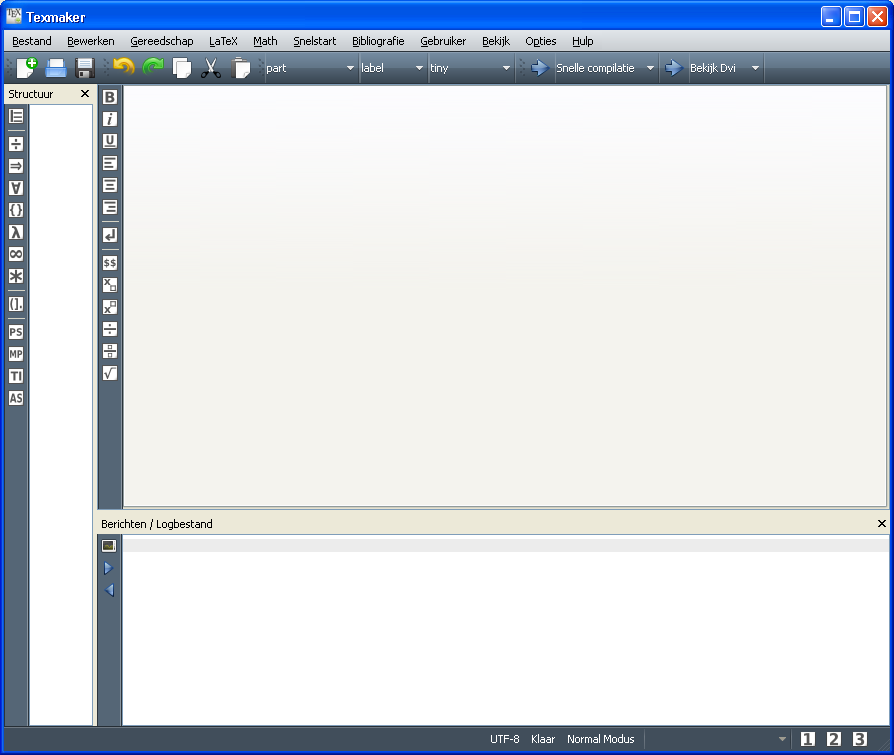
\includegraphics[scale=.2]{screenshot-1.png}
\end{frame}

\begin{frame}[fragile]
  \frametitle{Instellingen wijzigen}

  \begin{enumerate}
    \item ga naar Opties > Texmaker instellen
    \item plaats het volledige pad naar \texttt{pdflatex} bij PdfLaTeX
	  \begin{verbatim}
"C:/Program Files/MikTeX 2.9/miktex/bin/pdflatex.exe"
[...] -interaction=nonstopmode %.tex
	  \end{verbatim}
  \item plaats het volledige pad naar \texttt{bibtex} bij BibTex en verwijder \texttt{.aux}
	  \begin{verbatim}
"C:/Program Files/MikTeX 2.9/miktex/bin/bibtex.exe" %
	  \end{verbatim}
  \end{enumerate}
\end{frame}

\begin{frame}[fragile]
  \frametitle{Test}
  Typ volgende code over en druk op \texttt{F1}. Er zou iets moeten verschijnen.
  \inputminted{latex}{test-1.tex}
\end{frame}

\section{Wat u moet weten}
\begin{frame}
  \frametitle{Witruimte}
  Witruimte gedraagt zich \emph{niet} zoals in pakweg Microsoft Word. Enkele regels:
  \begin{itemize}
  	\item spaties, tabs en regeleindes zijn allemaal equivalent met \'e\'en spatie;
  	\item opeenvolgende witruimte wordt samengevoegd;
  	\item twee regeleindes na elkaar vormen = nieuwe alinea;
  	\item er zijn (uiteraard) uitzonderingen (zie~\texttt{verbatim}).
  \end{itemize}
\end{frame}

\begin{frame}[fragile]
  \frametitle{Speciale karakters}
  Zoals in andere programmeertalen zijn er bepaalde symbolen met een bepaalde betekenis: \verb|$ & % # _ { } ~ ^ \|

  De belangrijkste voor het moment zijn: \verb|\|, \verb|{|, \verb|}| en \verb|%|, voor commando's en commentaar.
\end{frame}

\begin{frame}[fragile]
  \frametitle{Speciale karakters: voorbeeld}

  \begin{minted}{tex}
\section{Voorbeeld}
Dit is een voorbeeldzin. % iets interessants schrijven

Dit is een~\emph{tweede} zin.
% commentaar op een nieuwe regel, \emph{test} doet niets
  \end{minted}

  \begin{exampleblock}{Aan de slag}
    Werk verder in je testdocument (tussen \texttt{\textcolor{uagreen}{\textbackslash begin}\{document\}} en \texttt{\textcolor{uagreen}{\textbackslash end}\{document\}}) en druk op \texttt{F1} als je klaar bent.
  \end{exampleblock}
\end{frame}

\begin{frame}[fragile]
  \frametitle{Escaping}

  Wat als we toch zo'n speciale karakters wensen te gebruiken? Door ze te prefixen met een~\verb|\|:

  \begin{tabular}[]{cc|cc|cc|cc}
    \verb|\$| & \$ & 
    \verb|\&| & \& &
    \verb|\%| & \% &
    \verb|\#| & \# \\ \\
    \verb|\_| & \_ &
    \verb|\{| & \{ &
    \verb|\}| & \}
  \end{tabular}

  En~\textbackslash~dan? Hiervoor gebruik je~\verb|\textbackslash|, je zou geneigd zijn om \verb|\\| te gebruiken maar dit heeft een speciale betekenis.
\end{frame}

\begin{frame}[fragile]
  \frametitle{Commando's}

  \begin{itemize}
	  \item begint met een backslash, gevolgd door een naam (enkel letters!);
	  \item hoofdlettergevoelig;
	  \item wordt be\"eindigd door een spatie (volgende tekst wordt er meteen achter geplaatst);
	  \item kan parameters meekrijgen (later meer).
  \end{itemize}

  \begin{LTXexample}[pos=r]
\LaTeX is leuk \\
\LaTeX~is leuk \\
\LaTeX{} is leuk
  \end{LTXexample}
\end{frame}

\begin{frame}
  \frametitle{Terug naar het testbestand}
  Dit zou je nog steeds ergens opgeslagen moeten hebben (eventueel terug leegmaken). Zo nee mag je het nogmaals overtypen.
  \inputminted{latex}{test-1.tex}
\end{frame}

\begin{frame}
  \frametitle{Nu wat uitgebreider}
  \inputminted{latex}{test-2.tex}
\end{frame}

\begin{frame}
  \frametitle{Structuur}

  \begin{description}
	\item[preamble] bevat de configuratie van het bestand, zie je niet rechtstreeks in de output
	  \begin{itemize}
      \item \texttt{\textcolor{uagreen}{\textbackslash documentclass}\{\}},
	  	\item packages,
	  	\item definities van commando's.
	  \end{itemize}
    \item[document] alles tussen~\texttt{\textcolor{uagreen}{\textbackslash begin}\{document\}} en~\texttt{\textcolor{uagreen}{\textbackslash end}\{document\}}, de eigenlijke tekst
  \end{description}
\end{frame}

\begin{frame}
  \frametitle{\texttt{\textbackslash documentclass\{\}}}

  \textcolor{uagreen}{\texttt{\textbackslash documentclass}}\{$\langle\textsl{class}\rangle$\}

  beschrijft het~\emph{soort} document, in \LaTeX~zijn (onder andere) voorzien:
  \begin{description}
	  \item[\texttt{article}] korte verslagen, artikels
	  \item[\texttt{report}] langere verslagen, cursussen
	  \item[\texttt{letter}] brieven (automatische hoofdingen, handtekeningen, etc.)
  \end{description}

  maar er zijn ook nog (onder meer)
  \begin{description}
	  \item[\texttt{memoir}] veel meer controle over layout
	  \item[\texttt{beamer}] voor slides (u ziet hier het resultaat)
  \end{description}
\end{frame}

\begin{frame}[fragile]
  \frametitle{\texttt{\textbackslash documentclass\{\}}: opties}

  \textcolor{uagreen}{\texttt{\textbackslash documentclass}}[$\langle\textsl{opties}\rangle$]\{$\langle\textsl{class}\rangle$\}

  \begin{description}
	  \item[\texttt{$\langle n\rangle$pt}] lettergrootte, default is~\texttt{10pt}, $n\in\left\{ 10,11,12 \right\}$
	  \item[\texttt{a4paper}] papierformaat, default is het Amerikaanse~\texttt{letterpaper}
	  \item[\texttt{titlepage}] zorgt voor een titelpagina, \texttt{article} default niet, \texttt{report} en~\texttt{book} wel, ook~\texttt{notitlepage}
	  \item[\ldots] 
  \end{description}

  Zie~\texttt{lshort-dutch} voor meer.
\end{frame}

\begin{frame}
  \frametitle{Uitgebreid voorbeeld met correcte opties}
  \inputminted{latex}{test-3.tex}
\end{frame}

\begin{frame}[fragile]
  \frametitle{Packages}
  Het wiel heruitvinden is nergens voor nodig, daarom zijn er packages die specifieke problemen oplossen.

  \textcolor{uagreen}{\texttt{\textbackslash usepackage}}\verb|[|$\langle\textsl{opties}\rangle$\verb|]{|$\langle\textsl{naam}\rangle$\verb|}|
\end{frame}

\begin{frame}[fragile]
  \frametitle{Voorbeelden van packages}

  \begin{description}
	\item[\texttt{babel}] bevat informatie over talen, meestal te gebruiken met optie~\texttt{[dutch]}
	\item[\texttt{amsmath}] maakt wiskunde schrijven makkelijker
	\item[\texttt{amsfonts}] wiskundige lettertypes: $\mathbb{R}$, $\mathfrak{m}$
	\item[\texttt{amssymb}] symbolen die met wiskunde te maken hebben (zie ook~\url{http://ctan.org/tex-archive/info/symbols/comprehensive}): $\varinjlim$, $\hookrightarrow$, \ldots
    \item[\texttt{graphicx}] werken met afbeeldingen
    \item[] \ldots
  \end{description}
\end{frame}

\begin{frame}[fragile]
  \frametitle{Gebruik van packages}

  \begin{alertblock}{Lawinegevaar}
    Gebruik enkel packages in je document die je daadwerkelijk nodig hebt, kopieer niet telkens dezelfde lijst om er dan nog aan toe te voegen. Je krijgt op den duur conflicten.
  \end{alertblock}

  Packages hebben vaak \emph{erg} goede documentatie, gebruik deze:

  \texttt{http://ctan.org/pkg/$\langle\textsl{naam}\rangle$}
  \pause
  \begin{exampleblock}{Oefening}
    Probeer dit voor \verb|amsmath|, \verb|pgf| en \verb|thmtools|.
  \end{exampleblock}
\end{frame}

\begin{frame}[fragile]
  \frametitle{Eigenlijke document}

  \begin{minted}{latex}
\begin{document}
% alles hiertussen vormt je document
\end{document}
  \end{minted}

  zal vaak een~\texttt{\textcolor{uagreen}{\textbackslash maketitle}} bevatten, de rest komt later
\end{frame}

\begin{frame}[fragile]
  \frametitle{Ons afgewerkte voorbeeld}
  \small
  \inputminted{latex}{test-4.tex}
\end{frame}

\section{Tekstopmaak}
\subsection{De structuur van tekst}
\begin{frame}[fragile]
  \frametitle{Lokale structuur}

  Alles draait om \emph{alinea's}. Een nieuwe alinea beginnen gebeurt door twee witregels te maken:

  \begin{minted}{latex}
Dit is een eerste alinea.

Dit is een tweede alinea.
Dit is geen derde alinea, de nieuwregel wordt genegeerd.
  \end{minted}

  Gebruik deze om je tekst lokaal structuur te geven.
\end{frame}

\begin{frame}
  \frametitle{Andere manieren voor lokale structuur}

  \begin{itemize}
    \item een regel afbreken (dus een nieuwe starten): \texttt{\textbackslash\textbackslash} of \texttt{\textcolor{uagreen}\textbackslash newline};
    \item een nieuwe pagina beginnen: \texttt{\textcolor{uagreen}{\textbackslash clearpage}} en \texttt{\textcolor{uagreen}{\textbackslash newpage}};
    \item nog wat varianten: zie \texttt{lshort-dutch}.
  \end{itemize}

  Een wijze raad: ik gebruik deze zo goed als nooit, er is geen reden om aan te nemen dat jullie ze \emph{wel} excessief nodig hebben, je doet misschien iets verkeerd in dat geval.
\end{frame}

\begin{frame}
  \frametitle{Opmerking bij \texttt{\textbackslash clearpage} en \texttt{\textbackslash newpage}}

  \begin{exampleblock}{De enige echte waarheid}
    \texttt{\textcolor{uagreen}{\textbackslash clearpage}} zorgt er voor dat tabellen en figuren die nog getypeset moeten worden geplaatst worden \emph{voor} de nieuwe pagina, bij \texttt{\textcolor{uagreen}{\textbackslash newpage}} gebeurt dit niet.
  \end{exampleblock}
  
  Er zijn ook \texttt{\textcolor{uagreen}{\textbackslash nopagebreak}[$\langle$\textsl{n}$\rangle$]}, \texttt{\textcolor{uagreen}{\textbackslash pagebreak}[$\langle$\textsl{n}$\rangle$]} en \texttt{\textcolor{uagreen}{\textbackslash nolinebreak}[$\langle$\textsl{n}$\rangle$]} die een bepaalde mate van het doorbreken der voorgeprogrammeerde regels bepalen.
\end{frame}

\begin{frame}
  \frametitle{Globale structuur}

  Om hoofdstukken en varianten aan te duiden gebruiken we
  \begin{tabular}{lcl}
    commando & niveau & opmerking \\\midrule
    \texttt{\textcolor{uagreen}{\textbackslash part}\{\}} & -1 & niet in~\texttt{letter} \\
    \texttt{\textcolor{uagreen}{\textbackslash chapter}\{\}} & 0 & niet in~\texttt{letter} en~\texttt{article} \\
	  \texttt{\textcolor{uagreen}{\textbackslash section}\{\}} & 1 & niet in~\texttt{letter} \\
    \texttt{\textcolor{uagreen}{\textbackslash subsection}\{\}} & 2 & niet in~\texttt{letter} \\
    \texttt{\textcolor{uagreen}{\textbackslash subsubsection}\{\}} & 3 & niet in~\texttt{letter} \\
    \texttt{\textcolor{uagreen}{\textbackslash paragraph}\{\}} & 4 & niet in~\texttt{letter} \\
	  \texttt{\textcolor{uagreen}{\textbackslash subparagraph}\{\}} & 5 & niet in~\texttt{letter} \\
  \end{tabular}
\end{frame}

\begin{frame}[fragile]
  \frametitle{Wat \emph{niet} te doen?}

  \begin{itemize}
	  \item zelf alinea's forceren met behulp van \verb|\\|;
    \item zelf met vette tekst, eigen nummeringen of wat dan ook structuur proberen aan te brengen;
    \item te veel niveaus gebruiken: ik heb nog nooit \texttt{\textcolor{uagreen}{\textbackslash subsubsection}\{\}} of \texttt{\textcolor{uagreen}{\textbackslash subparagraph}\{\}} gebruikt;
    \item \ldots
  \end{itemize}
\end{frame}

\begin{frame}[fragile]
  \frametitle{\texttt{\textbackslash tableofcontents}}
  \begin{minted}{latex}
\tableofcontents
  \end{minted}
  \LaTeX~maakt automatisch een inhoudsopgave op basis van de gebruikte~\texttt{\textcolor{uagreen}{\textbackslash section}\{\}}-commando's en aanverwanten.
  
  Om de diepte te controleren:
  \begin{minted}{latex}
\setcounter{tocdepth}{3}
  \end{minted}
\end{frame}

\begin{frame}[fragile]
  \frametitle{\texttt{\textbackslash tableofcontents}}

  \begin{exampleblock}{Tip}
    Voeg \texttt{\textcolor{uagreen}{\textbackslash usepackage}\{hyperref\}} toe aan je preamble om een inhoudsopgave in je \texttt{pdf} reader te krijgen.
  \end{exampleblock}
\end{frame}

\subsection{Speciale karakters en symbolen}
\begin{frame}[fragile]
  \frametitle{Aanhalingstekens}

  We willen als resultaat~``test'', gebruik hiervoor
  \begin{minted}{tex}
	``test''
  \end{minted}
  dus eerst back-ticks en daarna vertical quotes.
  \begin{alertblock}{Tip}
	Gebruik~\emph{nooit} \verb|"|. Het resultaat: "test".
  \end{alertblock}
\end{frame}

\begin{frame}[fragile]
  \frametitle{Enkele aanhalingstekens}

  Heel simpel: gewoon \'e\'en back-tick om te openen en \'e\'en vertical quote om te sluiten.

  \begin{LTXexample}[numbers=none,basicstyle=\ttfamily]
`test'
  \end{LTXexample}
\end{frame}

\begin{frame}[fragile]
  \frametitle{Liggende streepjes}
  Niet minder dan vi\'er soorten liggende streepjes:
  \begin{tabular}[]{cccc}
	naam & input & output & doel \\\midrule
	hyphen & \verb|-| & - & splitsen in lettergrepen \\
	en dash & \verb|--| & -- & reeksen jaartallen, pagina's, \ldots \\
	em dash & \verb|---| & --- & gedachtestreepje \\
	minteken & \verb|$-$| & $-$ & in wiskundige uitdrukking
  \end{tabular}
\end{frame}

\begin{frame}[fragile]
  \frametitle{Liggende streepjes: voorbeeld}

  \begin{minted}{latex}
vergeet-me-nietje, $n$-dimensionaal
pagina's 480--492, 1939--1945, de vlucht New York--London
Jan gaf de pennenzak --- inclusief slijper --- aan Tim.
Hoeveel is~$5-3$?
  \end{minted}
\end{frame}

\begin{frame}[fragile]
  \frametitle{Het beletselteken}
  
  Niet zo... maar zo\ldots (in dit lettertype maakt het weinig verschil, in andere gevallen w\'el)
  \begin{minted}{latex}
Niet zo... maar zo\ldots
  \end{minted}
\end{frame}

\begin{frame}[fragile]
  \frametitle{Accenten}

  \begin{center}
    \begin{tabular}{lllllllllll}
      \`o & \verb|\`o| & & \'o & \verb|\'o| & & \^o & \verb|\^o| & & \~o & \verb|\~o| \\
      \=o & \verb|\=o| & & \.o & \verb|\.o| & & \"o & \verb|\"o| & & \c c & \verb|\c| \\
	  \u o & \verb|\u o| & & \v o & \verb|\v o| & & \H o & \verb|H o| & & \c o & \verb|\c o| \\
	  \oe & \verb|\oe| & & \OE & \verb|\OE| & & \ae & \verb|\ae| & & \AE & \verb|\AE| \\
	  \o & \verb|\o| & & \O & \verb|\O| & & \l & \verb|\l| & & \L & \verb|\L| \\
	  \i & \verb|\i| & & \j & \verb|\j| & & !` & \verb|!`| & & ?` & \verb|?`|
    \end{tabular}
  \end{center}
\end{frame}

\begin{frame}[fragile]
  \frametitle{Accenten: de belangrijke}

  \begin{itemize}
    \item accent grave
      \begin{LTXexample}
\`a
      \end{LTXexample}
    \item accent aigu
      \begin{LTXexample}
\'e
      \end{LTXexample}
    \item c\'edille
      \begin{LTXexample}
\c c
      \end{LTXexample}
    \item trema
      \begin{LTXexample}
\"a \"e \"{e}
      \end{LTXexample}
  \end{itemize}
\end{frame}

\begin{frame}[fragile]
  \frametitle{Taal en woordsplitsing}

  Een klein uitstapje: herinner je de lessen Nederlands nog waar je leerde splitsen in lettergrepen? \LaTeX~doet dit automatisch voor je!

  \begin{enumerate}
    \item \texttt{\textcolor{uagreen}{\textbackslash usepackage}[dutch]\{babel\}}
    \item afbreking verhinderen: \texttt{\textcolor{uagreen}{\textbackslash mbox}\{\}}
    \item je kan het handmatig aanpassen indien nodig (bijvoorbeeld via \texttt{\textcolor{uagreen}{\textbackslash hyphenation}\{\}} en \texttt{\textcolor{uagreen}{\textbackslash discretionary}\{\}\{\}\{\}} of lokaal met~\verb|\-|), zie \texttt{lshort-dutch}
  \end{enumerate}
\end{frame}

\begin{frame}[fragile]
  \frametitle{Taal en woordsplitsing: voorbeelden}

  \begin{minted}{latex}
\hyphenation{Fortran wis-kun-de}
\discretionary{diner-}{tje}{dineetje}

elementaire\-deeltjes\-fysica\-fanaat
\mbox{bestand}
  \end{minted}
  Ik wijs je op het bestaan hiervan voor moest je ooit in een situatie komen waarbij het grondig fout loopt, maar ik heb het nog nooit nodig gehad.
\end{frame}


%\begin{frame}[fragile]
%  \frametitle{Font encoding}
%
%  Je kan de nodige accenten onthouden (wat makkelijker is dan je denkt), of je gebruikt
%  \begin{minted}{tex}
%\usepackage[T1]{fontenc}
%\usepackage{lmodern}
%  \end{minted}
%  of een ander lettertype naar keuze, zorg dat je voldoende fonts hebt.
%
%  Nu kan je gewoon accenten typen zoals je gewend bent.
%\end{frame}

\begin{frame}[fragile]
  \frametitle{Spatiegebruik}

  Er zijn drie soorten spaties: de gewone spatie \texttt{\textvisiblespace}, de tilde \texttt{\~} en \texttt{\textbackslash\textvisiblespace}. Gebruik de eerste bij gewone tekst, de tweede als non-breakable space en de derde wanneer een punt bij een afkorting geen einde van een zin aanduidt of na een commando (waarom?).

\begin{LTXexample}
gewone tekst \\
\LaTeX\ is leuk \\
ik zag 2~beren
\end{LTXexample}
\end{frame}

\begin{frame}
  \frametitle{Franse stijl}

  \LaTeX\ gebruikt een iets bredere spatie na het einde van een zin, wil je dit niet, gebruik dan \texttt{\textcolor{uagreen}{\textbackslash frenchspacing}}.
\end{frame}

\subsection{Verwijzingen}
\begin{frame}
  \frametitle{Verwijzingen}

  We kunnen verwijzen naar objecten met een nummer:
  \begin{itemize}
	  \item hoofdstukken,
	  \item figuren,
	  \item tabellen,
	  \item alinea's,
	  \item opsommingen,
	  \item \ldots
  \end{itemize}
\end{frame}

\begin{frame}[fragile]
  \frametitle{Markers}

  Maak een~\texttt{label} aan met~\texttt{\textcolor{uagreen}{\textbackslash label}\{$\langle$\textsl{marker}$\rangle$\}}. Een tip: voeg aan de marker toe wat voor type het is:
  \begin{minted}{tex}
	\label{fig:zeemeeuw}
	\label{figure:zeemeeuw}
	\label{enumerate:pythagoras-2}
  \end{minted}

  \begin{alertblock}{Figuren en tabellen}
    We weten nog niet hoe we deze maken, maar het label komt~\emph{na} de caption! Het commando~\texttt{\textcolor{uagreen}{\textbackslash label}\{\}} onthoudt enkel de laatst gegenereerde nummer.
  \end{alertblock}
\end{frame}

\begin{frame}[fragile]
  \frametitle{Verwijzen}

  Door \texttt{\textcolor{uagreen}{\textbackslash ref}\{$\langle$\textsl{marker}$\rangle$\}} en \texttt{\textcolor{uagreen}{\textbackslash pageref}\{$\langle$\textsl{marker}$\rangle$\}}, de eerste geeft een numerieke identificatie (het hoofdstuknummer, de opsomming, \ldots), de tweede de pagina waarop deze zich bevindt.

  \begin{exampleblock}{Two passes}
	  \LaTeX\ werkt hier met een two-pass systeem: je moet je document twee keer builden om het resultaat te zien: de eerste keer slaat hij op waar welke verwijzingen staan, de tweede keer kan hij ze ook weergeven.
  \end{exampleblock}
\end{frame}

\begin{frame}[fragile]
  \frametitle{Voorbeeld}
  \begin{minted}{tex}
\section{Meeuwen}
\label{sec:meeuw}
Meeuwen zijn vogels.
\section{Conclusie}
In Hoofdstuk~\ref{sec:meeuw} op pag.~\pageref{sec:meeuw}
zagen we dat meeuwen vogels zijn.
\end{minted}

  \begin{exampleblock}{Spatiegebruik}
	Merk op dat wat we geleerd hebben over spatiegebruik hier belangrijk is!
  \end{exampleblock}
\end{frame}

\begin{frame}[fragile]
  \frametitle{Voetnoten}

  Een simpel commando: \texttt{\textcolor{uagreen}{\textbackslash footnote}\{$\langle$\textsl{tekst}$\rangle$\}}.
  \begin{minted}{tex}
	Voetnoten\footnote{Zoals deze.} zijn
	populair bij \LaTeX-gebruikers.
  \end{minted}

  \begin{exampleblock}{Voetnotitis}
	  Overdrijf niet met voetnoten\footnote{Nee, \'echt niet.}.
  \end{exampleblock}

  Let ook goed op de interpunctie, zoals in het voorbeeld duidelijk wordt.
\end{frame}

\subsection{Stijl van het lettertype wijzigen}
\begin{frame}
  \frametitle{Nadruk}

  Er zijn verschillende manieren om nadruk te leggen: \underline{onderlijnen}, \textsl{schuin}, \textbf{vet} of gewoon~\emph{benadrukt}.

  \LaTeX\ weet zelf wat goed is, probeer dus niet je eigen wil op te dringen. Vette en onderlijnde tekst wordt afgeraden en wat als je binnen een schuingedrukt stuk tekst nog iets wil benadrukken?
\end{frame}

\begin{frame}[fragile]
  \frametitle{Nadruk: voorbeelden}
  \begin{LTXexample}
\underline{onderlijnd} \\
\textit{italic} \\
\textsl{slanted} \\
\textbf{vet} \\
\texttt{typewriter} \\
\emph{benadrukt}
  \end{LTXexample}
\end{frame}

\begin{frame}
  \frametitle{Slanted vs.\ italic}

  Slanted type is gewone tekst maar enigszins verbogen, italic is een ander font waarin dus de letters daadwerkelijk anders zijn. Mijn voorkeur ligt bij slanted.

  Dit is \textsl{slanted tekst} en dit \textit{is italic}. Zoals je ziet is er in dit lettertype spijtig genoeg geen verschil, maar laten we het eens zelf proberen.
\end{frame}

\begin{frame}[fragile]
  \frametitle{Waarom nu~\texttt{\textbackslash emph}?}

  \begin{minted}{tex}
	\emph{Dit is een benadrukte tekst,
	  \emph{let op} voor de extra nadruk}
  \end{minted}

  Deze situatie komt bijvoorbeeld voor als je stellingen en definities opschrijft, je je~\verb|quotation| omgeving aanpast, \ldots
\end{frame}

\subsection{Omgevingen}
\begin{frame}
  \frametitle{Omgevingen}
  We zagen reeds commando's, maar \LaTeX~ondersteunt ook grotere entiteiten:

  \texttt{\textcolor{uagreen}{\textbackslash begin}\{$\langle\textsl{naam}\rangle$\}\{$\langle\textsl{opties}\rangle$\}[$\langle\textsl{opties}\rangle$]}\\
  \hspace{2em}\ldots \\  
  \texttt{\textcolor{uagreen}{\textbackslash end}\{$\langle\textsl{naam}\rangle$\}}
  \pause\begin{exampleblock}{Opmerking}
	  De syntax zoals ik ze hier schets is niet helemaal wat er \'echt gebeurt, maar dit is (gelukkig voor jullie) geen cursus \TeX~hacken.
  \end{exampleblock}
\end{frame}

\begin{frame}
  \frametitle{Lijsten}

  We hebben 3 omgevingen voor lijsten:
  \begin{description}[\texttt{description}]
  	\item[\texttt{itemize}] ongenummerde opsomming
  	\item[\texttt{enumerate}] genummerde opsomming
  	\item[\texttt{description}] beschrijvingen (u ziet er \'e\'en)
  \end{description}
\end{frame}

\begin{frame}[fragile]
  \frametitle{\texttt{itemize}}

  \begin{LTXexample}
\begin{itemize}
  \item eerste item;
  \item tweede item;
  \item derde item

    Een nieuwe alinea.
\end{itemize}
  \end{LTXexample}
\end{frame}

\begin{frame}[fragile]
  \frametitle{\texttt{enumerate}}

  \begin{LTXexample}
\begin{enumerate}
  \item eerste item;
  \item tweede item;
  \item derde item

    Een nieuwe alinea.
\end{enumerate}
  \end{LTXexample}
\end{frame}

\begin{frame}[fragile]
  \frametitle{\texttt{description}}

  \begin{LTXexample}
\begin{description}
  \item[hond] kwijlend zoogdier
  \item[walvis] zeezoogdier
  \item[Willy] bekend kalf
\end{description}
  \end{LTXexample}

  \pause\begin{exampleblock}{Tijdsgewrocht}
    Merk op welke Woestijnvisreeks op het moment van opstellen populair was.
  \end{exampleblock}
\end{frame}

\begin{frame}
  \frametitle{Nesting}

  Deze lijsten kunnen meerdere niveaus diep gaan:
  \begin{enumerate}
	\item dit is een eerste item op het eerste niveau
	\item dit is een tweede item op het eerste niveau
	  \begin{itemize}
		\item dit is een eerste item op het tweede niveau
		\item en dit een tweede
	  \end{itemize}
	\item dit is een derde item op het eerste niveau
	  \begin{enumerate}
		\item we kunnen ook genummerd nesten
	  \end{enumerate}
  \end{enumerate}

  \begin{alertblock}{Waarschuwing}
	Overdrijf niet!
  \end{alertblock}
\end{frame}


\begin{frame}
  \frametitle{Uitlijnen}

  \begin{itemize}
    \item links uitlijnen: \texttt{\textcolor{uagreen}{\textbackslash begin}\{flushleft\}...\textcolor{uagreen}{\textbackslash end}\{flushleft\}}
    \item rechts uitlijnen: \texttt{\textcolor{uagreen}{\textbackslash begin}\{flushright\}...\textcolor{uagreen}{\textbackslash end}\{flushright\}}
    \item centreren: \texttt{\textcolor{uagreen}{\textbackslash begin}\{center\}...\textcolor{uagreen}{\textbackslash end}\{center\}}
  \end{itemize}
\end{frame}

\begin{frame}[fragile]
  \frametitle{Centreren bij tabellen of figuren}

  We hebben nog niet gezien hoe tabellen of figuren werken, maar hier is al \emph{a word of advice}:
  \begin{exampleblock}{\texttt{\textbackslash centering}}
    Gebruik de~\texttt{\textcolor{uagreen}{\textbackslash centering}} macro als je figuren of tabellen wil centreren, hier komt geen extra verticale witruimte bij.
  \end{exampleblock}
\end{frame}

\begin{frame}[fragile]
  \frametitle{Verbatim}

  Om tekst \emph{letterlijk} over te nemen heb je verbatim nodig: inline is dit~\texttt{\textcolor{uagreen}{\textbackslash verb}|...\textcolor{uagreen}{\textbackslash verb}|} waar~\verb!|! eender welk karakter behalve letters, een asterisk of een spatie mag zijn.

  \texttt{\textcolor{uagreen}{\textbackslash verb}*|twee  spaties|} geeft~\verb*|twee  spaties|.

  Grotere stukken doe je met een omgeving:
  \begin{minted}{tex}
\begin{verbatim}
  ...
\end{verbatim}
\end{minted}
\end{frame}

\begin{frame}[fragile]
  \frametitle{Heb ik dit nodig?}

  Bijvoorbeeld output van~\textsc{Matlab}, R. Voor code kan het ook gebruikt worden maar beter is om hier~\verb|listings| of~\verb|minted| te gebruiken.

  \pause\begin{exampleblock}{Laatste les}
    Is er hier interesse voor? Momenteel is er hier iets kleins over voorbereid.
  \end{exampleblock}
\end{frame}

\begin{frame}[fragile]
  \frametitle{Abstract}

  Een korte inhoud geven doe je simpelweg via
\begin{minted}{tex}
\begin{abstract}
  korte inhoud
\end{abstract}
\end{minted}
\end{frame}


\exercise

\part{Les 2}
\lecture
{We leren hoe we een bibliografie toevoegen aan onze tekst, hoe we figuren en tabellen gebruiken en op het einde vertel ik nog over hoe we werken met lettertypes en lettergroottes.}
{les-2}
\begin{frame}
  \frametitle{Vragen van vorige week}

  \begin{description}[tabellen uit Excel]
    \item[paginanummering] \texttt{\textcolor{uagreen}{\textbackslash pagestyle}} en \texttt{\textcolor{uagreen}{\textbackslash thispagestyle}};
    \item[lettertypes] wordt deze les besproken;
    \item[bad boxes] zie volgende slide;
    \item[tabellen uit Excel] wordt deze les besproken;
    \item[\texttt{\textcolor{uagreen}{\textbackslash parindent}}] zie opgave vorige week en Wikibooks
  \end{description}
\end{frame}

\begin{frame}
  \frametitle{Bad boxes}

  \LaTeX\ gaat zelf de optimale splitsing van zinnen bepalen, maar soms is er geen goede keuze mogelijk en maakt \LaTeX\ geen keuze: we krijgen een \emph{bad box}. Oplossingen:
  \begin{itemize}
    \item negeren;
    \item manueel hyphenaten;
    \item tekst herschrijven;
    \item \texttt{\textcolor{uagreen}{\textbackslash usepackage}\{microtype\}} (zie \package{microtype});
  \end{itemize}

  Gebruik \texttt{\textcolor{uagreen}{\textbackslash documentclass}[draft]\{$\langle$\textsl{class}$\rangle$\}} om een goed beeld te krijgen.
\end{frame}

\section{Bibliografie\"en}
\subsection{Bib\TeX}
\begin{frame}
  \frametitle{Bibliografiebeheer}

  Een van d\'e redenen om~\LaTeX\ te gebruiken is het goede beheer van referenties en bibliografie\"en. We gebruiken hiervoor~Bib\TeX. Dit is een extern programma dat output genereert die we kunnen gebruiken in~\LaTeX.
\end{frame}

\begin{frame}
  \frametitle{Concept}

  \begin{itemize}
	\item \'e\'en (of meerdere) bestanden waarin bibliografie\-informatie staat, onafhankelijk van de weergave;
    \item citeren gebeurt zoals we met~\texttt{\textbackslash label} en \texttt{\textbackslash ref} werkten, maar nu met~\texttt{\textbackslash cite};
	\item de layout van de bibliografie en de citaten is aanpasbaar en onafhankelijk van hoe we onze bibliografie hebben opgeslagen.
  \end{itemize}
\end{frame}

\begin{frame}
  \frametitle{\texttt{.bib} bestand}

  \begin{enumerate}
	\item bevat (delen van) de bibliografie;
	\item volgt een vaste structuur:

	  \texttt{@\textsl{$\langle$entry-type$\rangle$}\{\textsl{$\langle$key$\rangle$},\\
	  \ \ \textsl{$\langle$field-1$\rangle$} = \textsl{$\langle$value-1$\rangle$}, \\
	  \ \ \ldots \\
	  \ \ \textsl{$\langle$field-$n\rangle$} = \textsl{$\langle$value-$n\rangle$} \\
	  \}}
	  
	  en we zullen deze nu invullen.
  \end{enumerate}
\end{frame}

\begin{frame}
  \frametitle{Entry types}

  Bepaalt wat voor type het document heeft:
  \begin{itemize}
	\item \texttt{article}
	\item \texttt{book}
	\item \texttt{inbook}: een specifiek deel van een boek
	\item \texttt{misc}
	\item \texttt{proceedings}
	\item \ldots
  \end{itemize}
\end{frame}

\begin{frame}
  \frametitle{Bib\TeX\ voorbeeld}

\texttt{@book\{\textsl{$\langle$key$\rangle$},\\
\ \ \textsl{$\langle$field-1$\rangle$} = \textsl{$\langle$value-1$\rangle$}, \\
\ \ \ldots \\
\ \ \textsl{$\langle$field-$n\rangle$} = \textsl{$\langle$value-$n\rangle$} \\
\}}
\end{frame}

\begin{frame}
  \frametitle{Keys}

  Zoals met~\texttt{\textbackslash label\{\textsl{$\langle$key$\rangle$}\}} hebben we een unieke key nodig. Je kan deze opbouwen op basis van de auteur, het jaar van publicatie, de titel, \ldots\ Zorg dat het voor jou duidelijk is.
\end{frame}

\begin{frame}
  \frametitle{Bib\TeX\ voorbeeld}

\texttt{{@}book\{formalized-music,\\
\ \ \textsl{$\langle$field-1$\rangle$} = \textsl{$\langle$value-1$\rangle$}, \\
\ \ \ldots \\
\ \ \textsl{$\langle$field-$n\rangle$} = \textsl{$\langle$value-$n\rangle$} \\
\}}
\end{frame}

\begin{frame}[fragile]
  \frametitle{Velden en waarden}

  Elke entry bevat een aantal keys (of velden) met geassocieerde waarden, \emph{afhankelijk van het type}. Sommige zijn verplicht, anderen zijn optioneel. Enkele voorbeelden:
  \begin{itemize}
	\item \texttt{author}
	\item \texttt{title}
	\item \texttt{year}
	\item \ldots
  \end{itemize}
  \verb|author = "Iannis Xenakis"| \\
  \verb|title = "Formalized Music"|
\end{frame}

\begin{frame}
  \frametitle{Types en velden}

  \begin{description}
	\item[\texttt{article}] verplicht: \texttt{author}, \texttt{title}, \texttt{journal}, \texttt{year} \\
	  optioneel: \texttt{volume}, \texttt{number}, \texttt{pages}, \texttt{month}, \texttt{note}, \texttt{key}
	\item[\texttt{book}] verplicht: \texttt{author} of~\texttt{editor}, \texttt{title}, \texttt{publisher}, \texttt{year} \\
	  optioneel: \texttt{volume}, \texttt{series}, \texttt{address}, \texttt{edition}, \texttt{month}, \texttt{note}, \texttt{key}
	\item[\texttt{inbook}] verplicht: \texttt{author} of~\texttt{editor}, \texttt{title}, \texttt{chapter} of~\texttt{pages}, \texttt{publisher}, \texttt{year} \\
	  optioneel: \texttt{volume}, \texttt{series}, \texttt{address}, \texttt{edition}, \texttt{month}, \texttt{note}, \texttt{key}
  \end{description}
\end{frame}

\begin{frame}
  \frametitle{Types en velden (2)}

  \begin{description}[\texttt{proceedings}]
	\item[\texttt{misc}] verplicht: geen \\
	  optioneel: \texttt{author}, \texttt{title}, \texttt{howpublished}, \texttt{month}, \texttt{year}, \texttt{note}, \texttt{key}
	\item[\texttt{proceedings}] verplicht: \texttt{title}, \texttt{year} \\
	  optioneel: \texttt{editor}, \texttt{publisher}, \texttt{organization}, \texttt{address}, \texttt{month}, \texttt{note}, \texttt{key}
  \end{description}
\end{frame}

\begin{frame}
  \frametitle{Een overzicht graag}

  \small
  \url{http://newton.ex.ac.uk/tex/pack/bibtex/btxdoc/node6.html}, \url{http://newton.ex.ac.uk/tex/pack/bibtex/btxdoc/node7.html}
  {\ } \\
  {\ } \\
  \url{http://en.wikibooks.org/wiki/LaTeX/Bibliography_Management}
\end{frame}

\begin{frame}[fragile]
  \frametitle{Bib\TeX\ voorbeeld}

  \begin{minted}{tex}
@book{formalized-music,
  author = {Iannis Xenakis},
  title = {Formalized Music}
  publisher = {Pendragon Press},
  year = 2001,
  edition = {second},
  isbn = "978-1576470794"
}
  \end{minted}
\end{frame}

\begin{frame}[fragile]
  \frametitle{En websites?}

  In Bib\TeX\ geen concrete oplossing, wel een pseudo-oplossing:
  \begin{minted}{tex}
@misc{wiki:aardappel,
  author = {Wikipedia}
  title = {Aardappel},
  year = 2011,
  howpublished =
    {\url{http://nl.wikipedia.org/wiki/Aardappel}}
}
  \end{minted}
  Vergeet geen~\verb|\usepackage{url}| of (bij voorkeur) \verb|\usepackage{hyperref}|!
\end{frame}

\subsection{\LaTeX}
\begin{frame}[fragile]
  \frametitle{En nu?}

  Nu vertellen we~\LaTeX\ dat we met een bibliografie werken:
  \begin{minted}{tex}
\bibliographystyle{plain}
\bibliography{file-1,file-2}
\end{document}
  \end{minted}
  \begin{alertblock}{Spaties}
	Geen spatie tussen opeenvolgende bestanden gebruiken. Extensies zijn ook niet nodig.
  \end{alertblock}
\end{frame}

\begin{frame}[fragile]
  \frametitle{En we citeren}

  \begin{minted}{tex}
	Dit is een citaat, zie~\cite{wiki:bibtex}.
  \end{minted}
\end{frame}

\begin{frame}[fragile]
  \frametitle{Werkwijze}

  Herinner je het two-pass systeem voor verwijzingen? Nu hebben we een four-pass:
  \begin{verbatim}
pdflatex document.tex
bibtex document.aux
pdflatex document.tex
pdflatex document.tex\end{verbatim}
We proberen dit in \TeX maker.
\end{frame}

\begin{frame}[fragile]
  \frametitle{Na de eerste stap}
  \begin{verbatim}
LaTeX Warning: Citation `lamport94' on page 1 undefined
  on input line 21.
...
LaTeX Warning: There were undefined references.\end{verbatim}
\end{frame}

\begin{frame}[fragile]
  \frametitle{Na de tweede stap}
  \begin{verbatim}
This is BibTeX, Version 0.99c (Web2C 7.3.1)
The top-level auxiliary file: latex_source_code.aux
The style file: plain.bst
Database file #1: sample.bib\end{verbatim}
\end{frame}

\begin{frame}[fragile]
  \frametitle{Na de derde stap}
  \begin{verbatim}
LaTeX Warning: Label(s) may have changed.
Rerun to get cross-references right. 
  \end{verbatim}
\end{frame}

\begin{frame}
  \frametitle{In \TeX maker}

  Tijd voor experiment.
\end{frame}

\begin{frame}[fragile]
  \frametitle{Citeren in je eigen taal}

  \begin{minted}{tex}
\usepackage[fixlanguage]{babelbib}
\selectbiblanguage{dutch}

\bibliographystyle{babplain}
\bibliography{sample}
  \end{minted}
  Dus gebruik de juiste style.
\end{frame}

\begin{frame}[fragile]
  \frametitle{Uitgewerkt voorbeeld}

  \footnotesize
  \inputminted{tex}{bib-example.tex}
\end{frame}

\begin{frame}[fragile]
  \frametitle{Uitgewerkt voorbeeld}

  \inputminted{tex}{bib-example.bib}
\end{frame}

\begin{frame}[fragile]
  \frametitle{Mijn excuses}

  De package \package{babelbib} bevat nog bugs, ontdekte ik bij het maken van deze slides. Ik zal de maker contacteren om deze op te lossen. Tot dan moet je bijvoorbeeld je maanden meteen correct schrijven en editienummers voluit schrijven.
\end{frame}


\begin{frame}[fragile]
  \frametitle{Hack}

  \inputminted[firstline=9,lastline=19]{tex}{bib-example-extended.tex}
\end{frame}

\section{Tabellen en afbeeldingen}
\begin{frame}
  \frametitle{Idee}

  Tabellen en afbeeldingen kunnen rechtstreeks in onze tekst geplaatst worden, maar vaak is het beter dit in een float te plaatsen. Dit leg ik dus eerst uit, alvorens daadwerkelijk afbeeldingen en tabellen te maken.
\end{frame}

\subsection{Floats}
\begin{frame}
  \frametitle{Floats}

  De beste manier van opvullen wordt door \LaTeX\ zelf bepaald, de tekst vloeit rondom de figuren en tabellen om een optimale layout te bepalen. Je hebt zelf wel nog controle. \\[1em]

  \texttt{\textbackslash begin\{figure\}[$\langle$\textsl{modifiers}$\rangle$]} \\
  \texttt{\textbackslash end\{figure\}} \\[.5em]

  \texttt{\textbackslash begin\{table\}[$\langle$\textsl{modifiers}$\rangle$]} \\
  \texttt{\textbackslash end\{table\}}
\end{frame}

\begin{frame}
  \frametitle{Modifiers}

  \begin{tabular}{cl}
    code & betekenis \\\midrule
    \texttt{h} & plaats deze exact op de plaats van definitie \\
    \texttt{t} & bovenaan een pagina (top) \\
    \texttt{b} & onderaan een pagina (bottom) \\
    \texttt{p} & op een speciale pagina voor floats \\
    \texttt{!} & negeer eventuele betere opties
  \end{tabular}
\end{frame}

\begin{frame}[fragile]
  \frametitle{Voorbeeld}

  \begin{minted}{tex}
\begin{table}[h]
  ...
\end{table}

\begin{table}[p]
  ...
\end{table}
\end{minted}
\end{frame}

\begin{frame}
  \frametitle{Combinaties}

  Modifiers kunnen gecombineerd worden zodat je verschillende mogelijke opties toelaat: \\

  \begin{description}
    \item[\texttt{!hbp}] plaats de tabel op de plaats van definitie, onderaan een pagina of op een speciale pagina voor floats, ook al zou het beter zijn deze bovenaan een pagina te plaatsen
    \item[\texttt{tbp}] de standaardspecificatie
  \end{description}
\end{frame}

\begin{frame}[fragile]
  \frametitle{Opmerkingen}

  \begin{itemize}
    \item herinner \verb|\clearpage| versus \verb|\newpage|;
    \item floats worden in een wachtrij gezet die wordt gerespecteerd;
    \item probeer pas op het einde aandacht te besteden aan placement modifiers, als je tekst grotendeels af is.
  \end{itemize}
\end{frame}

\begin{frame}[fragile]
  \frametitle{Bijschriften}

  \texttt{\textbackslash begin\{figure\}[$\langle$\textsl{modifiers}$\rangle$]} \\
  \ \ \ldots \\
  \ \ \texttt{\textbackslash caption\{$\langle$\textsl{bijschrift}$\rangle$\}} \\
  \texttt{\textbackslash end\{figure\}}

  \begin{exampleblock}{Tip}
    Vergeet \verb|\usepackage[dutch]{babel}| niet!
  \end{exampleblock}
\end{frame}

\begin{frame}
  \frametitle{Verwijzen}

  Herinner de constructie met \texttt{\textbackslash label\{$\langle$\textsl{marker}$\rangle$\}} en \texttt{\textbackslash ref\{$\langle$\textsl{marker}$\rangle$\}}, deze werkt hier ook.

  \begin{alertblock}{Opgelet}
    Plaats het label \emph{binnenin} of \emph{na} de caption.
  \end{alertblock}
\end{frame}

\begin{frame}[fragile]
  \frametitle{Voorbeeld}
  \begin{minted}{tex}
\begin{figure}[tp]
  \centering
  \ldots
  \caption{Bijschrift}
  \label{figure:meeuw}
\end{figure}
\end{minted}
\end{frame}

\subsection{Afbeeldingen}
\begin{frame}[fragile]
  \frametitle{Afbeeldingen}

  Een belangrijke package:
  \begin{minted}{tex}
\usepackage{graphicx}
  \end{minted}
\end{frame}

\begin{frame}
  \frametitle{Ondersteunde formaten (voor \texttt{pdflatex})}

  \begin{description}[vectorformaten]
    \item[\texttt{jpg}] lossy, voor foto's (maar ik raad je dit af)
    \item[\texttt{png}] lossless, voor alles wat geen foto is zoals screenshots, diagrammen, schema's (een goede optie bij gebrek aan beter)
    \item[\texttt{pdf}] combineert voorgaande, maar ook echte vector graphics (het beste idee als het mogelijk is)
    \item[vectorformaten] de \emph{beste} optie, maar moeilijker
    \item[\texttt{eps}] via \texttt{epstopdf}
  \end{description}
\end{frame}

\begin{frame}[fragile]
  \frametitle{Afbeeldingen toevoegen}

  \texttt{\textbackslash includegraphics} \\
  \ \ \texttt{[$\langle$\textsl{optie-1}$\rangle$=$\langle$\textsl{waarde-1}$\rangle$,\ldots,$\langle$\textsl{optie-$n\rangle$}=$\langle$\textsl{waarde-$n\rangle$}]} \\
  \ \ \texttt{\{$\langle$\textsl{bestandsnaam}$\rangle$\}}

  \begin{minted}{tex}

\includegraphics[scale=0.5]{cat}
  \end{minted}

  \begin{exampleblock}{Extensie}
    Merk op: extensies zijn niet per se nodig.    
  \end{exampleblock}
\end{frame}

\begin{frame}[fragile]
  \frametitle{Opties}

  \begin{description}
    \item[\texttt{width}] en ook \texttt{height}, als er slechts \'e\'en gespecifieerd is schaalt de andere mooi mee
    \item[\texttt{scale=\textsl{$\langle$x$\rangle$}}] een schaalfactor, $x\in\mathbb{R}_0^+$
    \item[\texttt{angle=\textsl{$\langle$n$\rangle$}}] tegenwijzerzin draaien over~$n$ graden
  \end{description}

  De eenheden in \LaTeX\ werken zoals je zou verwachten:
  \begin{minted}{tex}

\includegraphics[width=3cm]{cat}

\includegraphics[width=1in,height=154pt]{cat}
\end{minted}

\href{http://en.wikibooks.org/wiki/LaTeX/Useful_Measurement_Macros}{\texttt{en.wikibooks.org/wiki/LaTeX/Useful\_Measurement\_Macros}}
\end{frame}

\begin{frame}[fragile]
  \frametitle{Nu samen met \texttt{figure}}

\begin{minted}{tex}
\begin{figure}[ht]
  \centering
  \includegraphics[width=3cm]{kitten}
  \caption{Een kat}
  \label{figure:cat}
\end{figure}
\end{minted}
\end{frame}

\subsection{Tabellen}
\begin{frame}[fragile]
  \frametitle{Opzet}

  We kennen al de \verb|table|-omgeving maar dat is slechts een wrapper rond tabellen, nu gaan we daadwerkelijk tabellen maken. Enkele opmerkingen:
  \begin{itemize}
    \item er is \emph{heel veel} mogelijk, ik kan verre van alles behandelen;
    \item probeer het simpel te houden: is je tabel nodig? is alle data nodig?
    \item er bestaan tools om tabellen te exporteren uit OpenOffice, dus misschien ook wel voor Microsoft Office.
  \end{itemize}
\end{frame}

\begin{frame}
  \frametitle{\texttt{tabular}}

  De omgeving waarin alles gebeurt, de vorm:

  \texttt{\textbackslash begin\{tabular\}[$\langle$\textsl{positie}$\rangle$]\{$\langle$\textsl{specificatie}$\rangle$\}} \\
  \ \ \texttt{\ldots} \\
  \texttt{\textbackslash end\{tabular\}}
\end{frame}

\begin{frame}[fragile]
  \frametitle{Positie}

  Niet heel erg van toepassing omdat je van mij altijd een \verb|table|-omgeving moet gebruiken, maar voor de volledigheid, hiermee wordt de positie tegenover de baseline gegeven, dus
  \begin{tabular}[b]{ccc}
    1 & 2 & 3 \\\midrule
    4 & 5 & 6
  \end{tabular}
  maar ook
  \begin{tabular}[c]{ccc}
    1 & 2 & 3 \\\midrule
    4 & 5 & 6
  \end{tabular}
  of
  \begin{tabular}[t]{ccc}
    1 & 2 & 3 \\\midrule
    4 & 5 & 6
  \end{tabular}
\end{frame}

\begin{frame}
  \frametitle{Specificatie, verticale informatie}

  Bepaalt het uitzicht van de tabel, is een reeks karakters met elk hun eigen betekenis die bepaalt hoeveel \emph{kolommen} er zijn, hoe deze uitgelijnd worden en waar er verticale lijnen geplaatst worden. \\[1em]

  \begin{tabular}{cl}
    specifier & werking \\\midrule
    \texttt{l} & links uitlijnen \\
    \texttt{c} & centreren \\
    \texttt{r} & rechts uitlijnen \\
    \texttt{|} & een verticale lijn (\texttt{||} zijn er twee) \\
    \texttt{p}\{$\langle$\textsl{breedte}$\rangle$\} & een alinea met een vaste breedte
  \end{tabular}
\end{frame}

\begin{frame}
  \frametitle{Verticale lijnen}

  \begin{alertblock}{Tip}
    Probeer verticale strepen te vermijden. Zie bijvoorbeeld ook de package \href{http://ctan.org/pkg/booktabs}{\texttt{ctan.org/pkg/booktabs}}.
  \end{alertblock}

  In deze slides gebruik ik deze package om meteen het goede voorbeeld te geven.
\end{frame}

\begin{frame}
  \frametitle{Hoe werkt \texttt{p}\{$\langle$\textsl{breedte}$\rangle$\}?}

  \begin{exampleblock}{Uitleg}
  Een cel wordt zo breed als nodig is, zonder rekening te houden met de breedte van het blad. Daarvoor dient de optie \texttt{p}\{$\langle$\textsl{breedte}$\rangle$\} dus.
\end{exampleblock}

  \begin{tabular}{cl}
    Een gecentreerde cel & Dit is een links uitgelijnde cel die botweg buiten het blad zal lopen. \\
  \end{tabular} \\[1em]
  \begin{tabular}{cp{.5\textwidth}}
    Een tweede tabel & Dit is een paragraaf die mooi wordt afgebroken zoals je kan zien. \\
  \end{tabular}
\end{frame}

\begin{frame}[fragile]
  \frametitle{Nieuwe manieren om afstanden te geven}

  We zagen reeds dat we via eenheden konden werken, maar \LaTeX\ specifieert ook een aantal lengtes afhankelijk van je document:
  \begin{minted}{tex}
\begin{tabular}{cp{.5\textwidth}}
  ...
\end{tabular}
  \end{minted}

  Zie wederom \href{http://en.wikibooks.org/wiki/LaTeX/Useful_Measurement_Macros}{\texttt{en.wikibooks.org/wiki/LaTeX/Useful\_Measurement\_Macros}}
\end{frame}

\begin{frame}[fragile]
  \frametitle{Horizontale informatie}

  \begin{tabular}{cp{.7\textwidth}}
    \texttt{\&} & tussen kolommen \\
    \texttt{\textbackslash\textbackslash} & start een nieuwe kolom \\
    \texttt{\textbackslash\textbackslash$\langle$\textsl{n}pt$\rangle$} & start een nieuwe kolom, optioneel een witruimte van de opgegeven dimensie \\
    \texttt{\textbackslash hline} & horizontale lijn \\
    \texttt{\textbackslash newline} & een nieuwe regel \emph{binnen de cel zelf}, voor \texttt{p\{$\langle$\textsl{dimensie}$\rangle$\}}
  \end{tabular} 

  En in de \package{booktabs}: \verb|\toprule|, \verb|\midrule|, \verb|\bottomrule|.
\end{frame}

\begin{frame}[fragile]
  \frametitle{Voorbeelden}

  \begin{LTXexample}
\begin{tabular}{lcr}
  1 & 2 & 3a \\
  4 & 5b & 6 \\
  7c & 8 & 9
\end{tabular} 
  \end{LTXexample}
\end{frame}

\begin{frame}[fragile]
  \frametitle{Voorbeeld}

  \inputminted{tex}{table-example.tex}
\end{frame}

\begin{frame}[fragile]
  \frametitle{Voorbeeld}

  \begin{tabular}{clp{.3\textwidth}}
  \toprule
  hoofding 1 & hoofding 2 & hoofding 3 \\\midrule
  item 1a & item 2a & item 3a \newline item 3a' \\
  item 1b & item 2b & item 3b \\
  item 1c & item 2c & item 3c \\
  \bottomrule
\end{tabular}

\end{frame}

\begin{frame}[fragile]
  \frametitle{\texttt{\textbackslash multicolumn}}

  \texttt{\textbackslash multicolumn\{$\langle$\textsl{n}$\rangle$\}\{$\langle$\textsl{specificatie}$\rangle$\}\{$\langle$\textsl{tekst}$\rangle$\}} \\[1em]

  \begin{tabular}{cl}
    $\langle$\textsl{n}$\rangle$ & aantal kolommen dat vanaf dan samengenomen moet worden \\
    $\langle$\textsl{specificatie}$\rangle$ & uitlijning, zoals daarvoor \\
    $\langle$\textsl{tekst}$\rangle$ & de eigenlijke tekst \\
  \end{tabular} \\[2em]

  Ook een package \package{multirow} om \verb|\multirow| mogelijk te maken.
\end{frame}

\begin{frame}[fragile]
  \frametitle{Alles te samen}

  \scriptsize
  \begin{minted}{tex}
\usepackage{dcolumn}
  \end{minted}
  \inputminted{tex}{table-example-2.tex}
\end{frame}

\begin{frame}
  \frametitle{Alles tesamen}

  \begin{table}[bp!]
  \centering
  \begin{tabular}{cD{.}{,}{-1}D{.}{.}{-1}}
    \toprule
    getal & \multicolumn{2}{c}{decimale voorstellingen} \\\midrule
    $\pi$ & 3.14 & 3.1415\ldots \\
    $e$ & 2.72 & 2.71\ldots \\
    $152/13$ & 11.70 & 11.6923077 \\
    \bottomrule
  \end{tabular}
  \caption{Een paar getallen binnen de wiskunde}
  \label{table:numbers}
\end{table}

\end{frame}

\section{Uitzicht}
\begin{frame}[fragile]
  \frametitle{Fontgrootte}

  Eerst en vooral: globaal via de opties van je documentclass.
\begin{minted}{tex}
\documentclass[a4paper,11pt]{article}
\end{minted}
\end{frame}

\begin{frame}[fragile]
  \frametitle{Lokaal wijzigingen aanbrengen}

  Er zijn 10 commando's die je tekst relatief tegenover de globale grootte wijzigen, gebruik deze dus het best.
\end{frame}

\begin{frame}[fragile]
\begin{tabular}{llll}
  \toprule
  size & 10pt (default) & 11pt option & 12pt option \\\midrule
  \verb|\tiny| &	6.80565 &	7.33325 &	7.33325 \\
  \verb|\scriptsize|& 	7.97224 &	8.50012& 	8.50012  \\
  \verb|\footnotesize|& 	8.50012 &	9.24994 &	10.00002 \\
  \verb|\small| 	&9.24994 &	10.00002 &	10.95003         \\
  \verb|\normalsize|& 	10.00002 &	10.95003 &	11.74988 \\
  \verb|\large| 	&11.74988 &	11.74988 &	14.09984         \\
  \verb|\Large| 	&14.09984 &	14.09984 &	15.84985         \\
  \verb|\LARGE| 	&15.84985 &	15.84985 &	19.02350         \\
  \verb|\huge| 	&19.02350 &	19.02350 &	22.82086         \\
  \verb|\Huge| 	&22.82086 &	22.82086 &	22.82086        \\
  \bottomrule
  \end{tabular}
\end{frame}

\begin{frame}
  \frametitle{Lettertypes}

  We stoten op een van de nadelen van \LaTeX, in de jaren '80 was nog niet alles zo flexibel als we nu gewend zijn. Spelen met verschillende lettertypes is in \LaTeX~niet zo gemakkelijk als we zouden willen.
\end{frame}

\begin{frame}
  \frametitle{Elk nadeel heb z'n voordeel}

  \begin{exampleblock}{Tip}
	Gebruik steeds zo weinig mogelijk verschillende (en exotische) lettertypes.
  \end{exampleblock}

  Mijn advies: verander je lettertype enkel globaal.
\end{frame}

\begin{frame}[fragile]
  \frametitle{En hoe dan te veranderen?}

  Het is niet mogelijk om de lettertypes uit je Windows- of Linuxinstallatie te gebruiken, enkel lettertypes waarvan \LaTeX~de informatie die het nodig heeft bezit kunnen werken.

  Daarnaast is het normaal gezien alleen maar mogelijk om \emph{globaal} te wijzigen. Een voorbeeld:
\begin{minted}{tex}
\usepackage[T1]{fontenc}
\usepackage{tgpagella}
\end{minted}
\end{frame}

\begin{frame}[fragile]
  \frametitle{En wat als ik toch lokale wijzigingen wil?}

  Gebruik KOMA-Script of \texttt{memoir}, dit zijn aparte document classes (zie vorige les) die veel meer flexibiliteit bieden.
\end{frame}

\begin{frame}
  \frametitle{En waar vind ik dan die lettertypes?}

  E\'en plek: \url{http://www.tug.dk/FontCatalogue/}
\end{frame}

\begin{frame}[fragile]
  \frametitle{\XeTeX}

  Dit is een uitbreiding op \LaTeX~die w\'el goed met lettertypes overweg kan. Maar ik ben er te weinig mee vertrouwd om er iets zinnig over te kunnen zeggen.
\end{frame}


\exercise

\part{Les 3}
\lecture
{We leren wiskunde en chemie typesetten.}
{les-3}
\begin{frame}
  \frametitle{Opmerkingen over vorige week}

  \begin{enumerate}
    \item Vaak kan je best Googlen naar de paper of het boek dat je wil citeren: je vindt dan automatisch bibliografische informatie;
  \end{enumerate}
\end{frame}
\section{Wiskunde}
\begin{frame}[fragile]
  \frametitle{Geschiedenis}

  Een van \emph{de} redenen om \TeX\ te ontwikkelen: tot de jaren '80 was het onmogelijk om zelf goed wiskunde te typesetten.

  De American Mathematical Society heeft een hoop werk geleverd in de jaren '90, met als resultaat:
  \begin{minted}{tex}
\usepackage{amsmath}
  \end{minted}

  \begin{exampleblock}{Andere omgevingen}
    Ik ga enkel \package{amsmath} omgevingen gebruiken, er zijn ook \TeX\ en \LaTeX-varianten maar deze zijn niet per se nodig.
  \end{exampleblock}
\end{frame}

\begin{frame}[fragile]
  \frametitle{Math mode}

  Normaal gezien houdt \LaTeX\ zich bezig met het typesetten van doorlopende tekst (dus in \emph{text mode}), omdat wiskunde zo'n fundamenteel andere aanpak vereist moetten we \LaTeX\ vertellen dat we naar \emph{math mode} willen.
  
  \inputminted{tex}{math-example.tex}
\end{frame}

\begin{frame}
  \frametitle{Het resultaat}

  In doorlopende tekst: $a^2+b^2=c^2$.

\begin{equation}
  f^{(n)}(a)=\frac{n!}{2\pi i}\oint_{\Gamma}
  \frac{f(\zeta)}{(\zeta-z)^{n+1}}\mathrm{d}\zeta
\end{equation}


  De eerste is \emph{inline} (of in \emph{text style}), de andere is in \emph{display style}.
\end{frame}

\begin{frame}[fragile]
  \frametitle{Spatiegebruik en de rol van letters}

  \begin{enumerate}
    \item spaties en regeleindes worden \emph{volledig} genegeerd (waar mogelijk), witruimte in formules komt door de semantiek van symbolen of handmatig;
    \item gewone letters zijn variabelen en worden dus in italic geplaatst.
      \begin{LTXexample}
$dit klopt niet$ \\
$f_{\text{int}}$
      \end{LTXexample}
  \end{enumerate}
\end{frame}

\subsection{Binnen math mode}
\begin{frame}[fragile]
  \frametitle{Grieks alfabet}

  Heel simpel:\\
  \texttt{\textbackslash$\langle$\textsl{letter}$\rangle$} en \texttt{\textbackslash$\langle$\textsl{Letter}$\rangle$}

  \begin{LTXexample}
$\alpha\beta\Gamma\Delta$
  \end{LTXexample}

  \begin{alertblock}{A tiny catch}
    Sommige Griekse hoofdletters zijn hetzelfde als de Latijnse, deze hebben dus geen aparte letter. Er is dus geen \verb|\Alpha| of \verb|\Chi|.
  \end{alertblock}
\end{frame}

\begin{frame}[fragile]
  \frametitle{Varianten}

  Voor de liefhebber, een paar varianten (de drie eerste zijn frequent, de rest niet):

  \begin{LTXexample}
$\epsilon\,\varepsilon$ \\
$\theta\,\vartheta$ \\
$\phi\,\varphi$ \\
$\pi,\varpi$ \\
$\rho\,\varrho$ \\
$\sigma\,\varsigma$
  \end{LTXexample}
\end{frame}

\begin{frame}[fragile]
  \frametitle{Operators}

  Ook wel ``functies met een naam''. Zoals daar zijn $\cos$, $\sin$, $\log$, \ldots

  \begin{LTXexample}
$\sin(\pi)=0$,
$\tan(\pi/2)=1$.
  \end{LTXexample}

  De meest voor de hand liggende zijn voor gedefinieerd, anders: \\
  \texttt{\textcolor{uagreen}{\textbackslash DeclareMathOperator}\textbackslash\textsl{$\langle$commandonaam$\rangle$}\{\textsl{$\langle$naam$\rangle$}\}}
  \begin{minted}{tex}
\DeclareMathOperator\characteristic{char}
\DeclareMathOperator\trace{tr}
\end{minted}
\end{frame}

\begin{frame}[fragile]
  \frametitle{Subscript mogelijk maken}

  \begin{LTXexample}
\begin{equation}
  \lim_{x\rightarrow 0}
  \frac{\sin x}{x}
\end{equation}
  \end{LTXexample}

  \texttt{\textcolor{uagreen}{\textbackslash DeclareMathOperator}\textbackslash\textsl{$\langle$commandonaam$\rangle$}\{\textsl{$\langle$naam$\rangle$}\}}
  \begin{minted}{tex}
\DeclareMathOperator*{\argmax}{arg\,max} 
\DeclareMathOperator*\argmax{arg\,max} 
  \end{minted}
\end{frame}

\begin{frame}[fragile]
  \frametitle{Sub- en superscript}

  Daarom zijn \verb|_| en \verb|^| dus speciale karakters:
  \small
  \begin{LTXexample}
$F_{n+2}=F_{n+1}+F_n$ \\
$O(n^{n^n})$ \\
$f|_{[0,1]}$ \\
$\lim_{x\rightarrow 0}$
\begin{equation}
  \int_0^x\!f'(x)\,\mathrm{d}x
\end{equation}
  \end{LTXexample}
\end{frame}

\begin{frame}[fragile]
  \frametitle{Breuken en binomiaalco\"effici\"enten}

  \texttt{\textcolor{uagreen}{\textbackslash frac}\{$\langle$\textsl{p}$\rangle$\}\{$\langle$\textsl{q}$\rangle$\}} en \texttt{\textcolor{uagreen}{\textbackslash binom}\{$\langle$\textsl{p}$\rangle$\}\{$\langle$\textsl{q}$\rangle$\}}

  \begin{LTXexample}
$\frac{\sin(x)}{\cos(x)}$ \\
$\binom{n}{k}$ \\
$\displaystyle\binom{n}{k}$
\begin{equation}
  \frac{\sin(x)}{\cos(x)}
\end{equation}
  \end{LTXexample}
  Of met~\package{xfrac}: $\sfrac{1}{2}$.
\end{frame}

\begin{frame}[fragile]
  \frametitle{\texttt{\textbackslash displaystyle}}

  Er zijn 4 formaten, van groot naar klein: \texttt{\textcolor{uagreen}{\textbackslash displaystyle}}, \texttt{\textcolor{uagreen}{\textbackslash textstyle}}, \texttt{\textcolor{uagreen}{\textbackslash scriptstyle}}, \texttt{\textcolor{uagreen}{\textbackslash scriptscriptstyle}}. Respectievelijk in display mode (in equations etc.), text mode (inline, of binnen omgevingen in equations), eerste niveau van sub- en superscripts, alle volgende niveaus van sub- en superscript.
\end{frame}

\begin{frame}[fragile]
  \frametitle{Wortels}

  \begin{LTXexample}
$\sqrt{2}$,~$\sqrt[3]{n}$
\begin{equation}
  \sqrt{\frac{3}{5}}
\end{equation}
  \end{LTXexample}
\end{frame}

\begin{frame}[fragile]
  \frametitle{Sommen en aanverwanten}

  \small
\begin{LTXexample}
$\sum_{k=1}^n k^2$ \\
\begin{equation}
  \sum_{k=1}^n k^2
  \bigotimes \coprod
  \oint \iiint
\end{equation}
\end{LTXexample}

\begin{alertblock}{\texttt{\textbackslash big}-varianten}
  Leer op de goede momenten \texttt{\textcolor{uagreen}{\textbackslash} bigcup} gebruiken. Want $\bigcup_{i=1}^n U_i\neq \cup_{i=1}^n U_i$.
\end{alertblock}
\end{frame}

\begin{frame}[fragile]
  \frametitle{\texttt{\textbackslash substack\{\}}}

  \begin{minted}{tex}
\begin{equation}
  \sum_{\substack{0<k<m \\ 0<l<n}} k+l
\end{equation}
  \end{minted}
\begin{equation}
  \sum_{\substack{0<k<m \\ 0<l<n}} k+l
\end{equation}
\end{frame}

\begin{frame}[fragile]
  \frametitle{\texttt{\textbackslash mathclap\{\}}}

  \begin{minted}{tex}
\begin{equation}
  \sum_{\mathclap{\substack{0<k<m \\ 0<l<n}}}\,k+l
\end{equation}
  \end{minted}
\begin{equation}
  \sum_{\mathclap{\substack{0<k<m \\ 0<l<n}}}\,k+l
\end{equation}
\end{frame}

\begin{frame}[fragile]
  \frametitle{Haakjes}

  \begin{LTXexample}
$(\cdot) \, [\cdot] \,$
$\{\cdot\}\, |\cdot| \,$
$\|\cdot\| \,$
$\langle\cdot\rangle \,$
$\lfloor\cdot\rfloor \,$
$\lceil\cdot\rceil$
  \end{LTXexample}
\end{frame}

\begin{frame}[fragile]
  \frametitle{Automatisch aanpassen}

  \begin{minted}{tex}
\begin{gather}
  \left( \frac{1}{2} \right) \\
  \left\{ x\in\mathbb{Q} \middle| x<\frac{1}{2} \right\}
\end{gather}
\end{minted}
\begin{gather}
  \left( \frac{1}{2} \right) \\
  \left\{ x\in\mathbb{Q} \,\middle|\, x<\frac{1}{2} \right\}
\end{gather}
\end{frame}

\begin{frame}[fragile]
  \frametitle{Matrices}

  \begin{minted}{tex}
\begin{gather}
  \begin{matrix} 1 & 0 \\ 0 & 1 \end{matrix} \quad
  \begin{pmatrix} 1 & 0 \\ 0 & 1 \end{pmatrix}
\end{gather}
  \end{minted}
\begin{gather}
  \begin{matrix} 1 & 0 \\ 0 & 1 \end{matrix} \quad
  \begin{pmatrix} 1 & 0 \\ 0 & 1 \end{pmatrix}
\end{gather}

Maar er zijn ook nog \verb|bmatrix|, \verb|Bmatrix|, \verb|vmatrix| en \verb|Vmatrix|. Ook is er telkens een \texttt{\textsl{$\langle$d$\rangle$}matrix*}-variant om alignment te bepalen.
\end{frame}

\begin{frame}[fragile]
  \frametitle{Grote matrices}
  
  \footnotesize
  \begin{minted}{tex}
\begin{gather}
  A_{m,n} =
    \begin{pmatrix}
      a_{1,1} & a_{1,2} & \cdots & a_{1,n} \\
      a_{2,1} & a_{2,2} & \cdots & a_{2,n} \\
      \vdots  & \vdots  & \ddots & \vdots  \\
      a_{m,1} & a_{m,2} & \cdots & a_{m,n}
    \end{pmatrix} 
\end{gather}
  \end{minted}
\begin{gather}
  A_{m,n} =
    \begin{pmatrix}
      a_{1,1} & a_{1,2} & \cdots & a_{1,n} \\
      a_{2,1} & a_{2,2} & \cdots & a_{2,n} \\
      \vdots  & \vdots  & \ddots & \vdots  \\
      a_{m,1} & a_{m,2} & \cdots & a_{m,n}
    \end{pmatrix} 
\end{gather}
\end{frame}

\begin{frame}[fragile]
  \frametitle{Tekst}

  Wat niet te doen:
  \begin{LTXexample}
$\dim_{Goldie}$
  \end{LTXexample}
  maar wel:
  \begin{LTXexample}
$\dim_{\text{Goldie}}$
  \end{LTXexample}

  Ook formatted text (zie eerste les).
\end{frame}

\begin{frame}
  \frametitle{Wiskundige lettertypes}

  \texttt{\textcolor{uagreen}{\textbackslash mathnormal}\{\}}, \texttt{\textcolor{uagreen}{\textbackslash mathrm}\{\}}, \texttt{\textcolor{uagreen}{\textbackslash mathit}\{\}} en \texttt{\textcolor{uagreen}{\textbackslash mathbf}\{\}} doen wat ze suggereren.

  \begin{description}
    \item[\texttt{\textcolor{uagreen}{\textbackslash mathsf}\{\}}] sans-serif, $\text{$k$-}\mathsf{Vect}$ (maar nu zie je weinig)
    \item[\texttt{\textcolor{uagreen}{\textbackslash mathcal}\{\}}] calligraphic, $\mathcal{O}$
    \item[\texttt{\textcolor{uagreen}{\textbackslash mathfrak}\{\}}] Fraktur, $\mathfrak{m}$
    \item[\texttt{\textcolor{uagreen}{\textbackslash mathbb}\{\}}] blackboard bold, $\mathbb{R}$
  \end{description}

  De laatste twee zitten verstopt in \package{amsfonts}.
\end{frame}

\begin{frame}[fragile]
  \frametitle{Accenten}

  Nu geen constructies meer met backslashes en obscure symbolen, maar dingen van de vorm \texttt{\textcolor{uagreen}{\textbackslash hat}\{\textsl{$\langle$x$\rangle$}\}}, \texttt{\textcolor{uagreen}{\textbackslash widehat}\{\textsl{$\langle$xyz$\rangle$}\}} en \texttt{\textcolor{uagreen}{\textbackslash overline}\{\textsl{$\langle$xyz$\rangle$}\}} wat resulteert in $\hat{x}$, $\widehat{xyz}$ en $\overline{xyz}$.

  De gewone weglatingstekens gelden nog wel: \verb|x'| levert $x'$.
\end{frame}

\begin{frame}
  \frametitle{Horizontale ruimte}

  Als basis: \texttt{\textcolor{uagreen}{\textbackslash quad}} is gelijk aan de fontgrootte, dus 10 tot 12 punt. \texttt{\textcolor{uagreen}{\textbackslash qquad}} is dit twee keer.

  Kleiner:
  \begin{description}
    \item[\texttt{\textbackslash,}] 3/18 quad
    \item[\texttt{\textbackslash:}] 4/18 quad
    \item[\texttt{\textbackslash;}] 5/18 quad
    \item[\texttt{\textbackslash!}] -3/18 quad
  \end{description}

  \begin{equation}
    \oint_\Gamma \zeta(x)\,\mathrm{d}x
  \end{equation}
\end{frame}

\begin{frame}
  \frametitle{Puntjes}

  In alle soorten en maten: \texttt{\textcolor{uagreen}{\textbackslash dots}}, \texttt{\textcolor{uagreen}{\textbackslash ldots}}, \texttt{\textcolor{uagreen}{\textbackslash cdots}}, \texttt{\textcolor{uagreen}{\textbackslash vdots}}, \texttt{\textcolor{uagreen}{\textbackslash ddots}}.

  {\ }

  Er zijn ook semantische varianten, \texttt{\textcolor{uagreen}{\textbackslash dotsc}} (komma's), \texttt{\textcolor{uagreen}{\textbackslash dotsb}} (binaire operaties), \texttt{\textcolor{uagreen}{\textbackslash dotsm}} (multiplicatie), \texttt{\textcolor{uagreen}{\textbackslash dotsi}} (integraal), \texttt{\textcolor{uagreen}{\textbackslash dotso}} (de rest).
\end{frame}

\begin{frame}[fragile]
  \frametitle{Symbolen}

  \emph{Bijna} elk gekend symbool in de wiskunde heeft een bepaald commando:
  \small
  \begin{LTXexample}
$\leq$, $\subseteq$, $\perp$
  \end{LTXexample}

  \normalsize
  Zij die niet in standaard \TeX\ zitten zijn wel in een package te vinden dan: The Comprehensive \LaTeX\ Symbol List. Vind je het niet zo gauw? Hulde voor \url{http://detexify.kirelabs.org}.
\end{frame}

\begin{frame}
  \frametitle{Oefening}

  Zoek volgende symbolen op en typeset ze:
  \begin{itemize}
	\item $\Gamma$
	\item $\subsetneqq$
	\item $\triangleleft$
	\item $\varinjlim$ (injectieve limiet)
	\item $\boxplus$
  \end{itemize}
\end{frame}

\begin{frame}[fragile]
  \frametitle{Pijlen}

  \texttt{\textcolor{uagreen}{\textbackslash}$\langle$\textsl{lengte}$\rangle\langle$\textsl{richting}$\rangle$\textcolor{uagreen}{arrow}}

  \begin{description}
    \item[\textsl{richting}] \texttt{right}, \texttt{left}, \texttt{up}, \texttt{down}
    \item[\textsl{lengte}] voeg \texttt{long} toe indien nodig
  \end{description}

  Wil je een dubbele pijl? Zet de eerste letter in hoofdletters.
  \begin{LTXexample}
$\rightarrow\ \uparrow\ $
$\leftarrow\ \downarrow$ \\
$\Rightarrow$
$\longleftarrow$
$\Leftrightarrow$
  \end{LTXexample}
\end{frame}


\subsection{Omgevingen}
\begin{frame}[fragile]
  \frametitle{Allemaal goed en wel\ldots}

  maar hoe geef ik nu wiskunde in? Je zag al wat hints: inline gebruiken we \verb|$...$| en er is zoiets als
  \begin{minted}{tex}
\begin{equation}
  ...
  \label{equation:...}
\end{equation}
  \end{minted}
\end{frame}

\begin{frame}[fragile]
  \frametitle{Een overzicht}

  \begin{description}
    \item[\texttt{equation}] een losstaande vergelijking
    \item[\texttt{align}] een reeks uitdrukkingen die uitgelijnd worden
    \item[\texttt{gather}] een reeks uitdrukkingen
  \end{description}

  De varianten met een ster laten de nummering vallen.
\end{frame}

\begin{frame}[fragile]
  \frametitle{\texttt{align} voorbeeld}

  \footnotesize
  \begin{minted}{tex}
\begin{align*}
  (x-y)^3&=(x-y)(x-y)^2 \\
  &=(x-y)(x^2-2xy+y^2) \\
  &=x^3-3x^2y+3xy^2-3y^3
\end{align*}
  \end{minted}
\begin{align*}
  (x-y)^3&=(x-y)(x-y)^2 \\
  &=(x-y)(x^2-2xy+y^2) \\
  &=x^3-3x^2y+3xy^2-3y^3
\end{align*}

Je kan ook meerdere alignments characters gebruiken.
\end{frame}

\begin{frame}[fragile]
  \frametitle{Verwijzen}

  Het gekende truukje met \texttt{\textcolor{uagreen}{\textbackslash label}\{\}} maar nu met \texttt{\textcolor{uagreen}{\textbackslash eqref}}.

  En als je wil herstarten met nummeren:
  \begin{minted}{tex}
\numberwithin{equation}{section}
  \end{minted}
\end{frame}

\begin{frame}[fragile]
  \frametitle{\texttt{cases}}

  Stuksgewijze definities:
  \begin{minted}{tex}
\begin{equation}
 u(x) =
  \begin{cases}
    \exp{x} & \text{voor $x\geq 0$} \\
    1 & \text{voor $x<0$}
  \end{cases}
\end{equation}
  \end{minted}
\begin{equation}
 u(x) =
  \begin{cases}
    \exp{x} & \text{if $x\geq 0$} \\
    1 & \text{if $x < 0$}
  \end{cases}
\end{equation}
\end{frame}

\begin{frame}[fragile]
  \frametitle{Stellingen}

  Voor al uw stellingen: \'e\'en package, \package{amsthm}.

  \texttt{\textcolor{uagreen}{\textbackslash newtheorem}\{$\langle$\textsl{omgeving}$\rangle$\}[$\langle$\textsl{nummering}$\rangle$]\{$\langle$\textsl{naam}$\rangle$\}} en \texttt{\textcolor{uagreen}{\textbackslash newtheorem}\{$\langle$\textsl{omgeving}$\rangle$\}\{$\langle$\textsl{naam}$\rangle$\}}[$\langle$\textsl{reset}$\rangle$]

  \begin{minted}{tex}
\newtheorem{theorem}{Stelling}[section]
\newtheorem{corollary}[theorem]{Gevolg}
\newtheorem{definition}[theorem]{Definitie}
\newtheorem{example}[theorem]{Voorbeeld}
\newtheorem{lemma}[theorem]{Lemma}
\newtheorem{remark}[theorem]{Opmerking}
  \end{minted}
\end{frame}

\begin{frame}[fragile]
  \frametitle{Opmerkingen bij \package{amsthm}}

  \begin{itemize}
    \item drie stijlen, \texttt{\textcolor{uagreen}{\textbackslash theoremstyle}\{definition\}};
    \item er is ook een omgeving voor bewijzen:
      {\footnotesize
      \begin{minted}{tex}
\begin{theorem}[Stelling van Pythagoras]
  $a^2+b^2=c^2$.

  \begin{proof}
    Triviaal.  
  \end{proof}
\end{theorem}
      \end{minted}
      }
    \item \texttt{\textcolor{uagreen}{\textbackslash numberswapping}}
  \end{itemize}
\end{frame}
  

\section{Chemie}
\begin{frame}
  \frametitle{Disclaimer}

  Ik ben geen chemicus, bijgevolg is mijn ervaring eerder beperkt (om niet te zeggen onbestaande). Als ik onzin uitkraam, gelieve me daar op te wijzen.

  Deze slides zijn dus ook maar een korte introductie.
\end{frame}

\subsection{Chemische formules}
\begin{frame}[fragile]
  \frametitle{\package{mhchem}}

  \begin{minted}{tex}
\ce{H2O}, \ce{[AgCl2]-}, \ce{1/2H2O}, \ce{^{227}_{90}Th+}
  \end{minted}
  resulteert in \ce{H2O}, \ce{[AgCl2]-}, \ce{1/2H2O}, \ce{^{227}_{90}Th+}
  \begin{minted}{tex}
\ce{CO2 + C -> 2CO}, \ce{CO2 + C ->[\alpha][\beta] 2CO}
  \end{minted}
  resulteert in \ce{CO2 + C -> 2CO}, \ce{CO2 + C ->[\alpha][\beta] 2CO}
\end{frame}

\begin{frame}[fragile]
  \frametitle{Groter voorbeeld}

  \small
  \begin{minted}{tex}
\ce{Zn^2+
  <=>[\ce{+ 2OH-}][\ce{+ 2H+}]
  $\underset{\text{zinkaation}}{\ce{Zn(OH)2 v}}$
  <=>C[+2OH-][{+ 2H+}]
  $\underset{\text{tetrahydroxozinkaation}}{\cf{[Zn(OH)4]^2-}}$
}
  \end{minted}
  \normalsize
\ce{Zn^2+
  <=>[\ce{+ 2OH-}][\ce{+ 2H+}]
  $\underset{\text{zinkaation}}{\ce{Zn(OH)2 v}}$
  <=>C[+2OH-][{+ 2H+}]
  $\underset{\text{tetrahydroxozinkaation}}{\cf{[Zn(OH)4]^2-}}$
}
\end{frame}

\begin{frame}[fragile]
  \frametitle{Werking}

  Er is een \texttt{\textcolor{uagreen}{\textbackslash ce}\{\}}-commando dat op een heel natuurlijke wijze chemische reacties interpreteert. Je hoeft geen math mode te gebruiken maar voor bijvoorbeeld sub- en superscripts is gebeurt dit wel standaard (dus gebruik \texttt{\textcolor{uagreen}{\textbackslash text}\{\}} indien nodig).

  Om chemische formules binnen wiskundeomgevingen te gebruiken: \texttt{\textcolor{uagreen}{\textbackslash cee}\{\}}.

  \begin{minted}{tex}
\usepackage[version=3]{mhchem}
  \end{minted}
\end{frame}


\subsection{Chemische structuren}
\begin{frame}
  \frametitle{Chemische structuren}

  Een paar mogelijkheden: \package{xymtex}, \package{ppchtex} of \package{tikz}. En er is \package{chemstyle} voor de consistentie.

  Een andere mogelijkheid: tekenen in pakweg ChemDraw en exporteren naar \texttt{pdf}.
\end{frame}


\subsection{SI-eenheden}
\begin{frame}
  \frametitle{\package{siunitx}}

  De meest recente package voor consistent werken met eenheden. Ik weet niet of deze werkt op de pc's hier, maar we bekijken de documentatie eens.
\end{frame}



\part{Les 4}
\lecture
{We leren code typesetten en presentaties maken.

Voor de liefhebbers is er vandaag geen opdracht, maar meer interactiviteit tijdens de les.}
{les-4}
\section{Code}
\begin{frame}
  \frametitle{Waarom code typesetten?}

  Ik denk dat zowat elke wetenschapsstudent wel eens met code in aanraking komt: Matlab, R, \LaTeX, \cpp, \ldots

  Net zoals we \LaTeX\ schrijven in een editor met mooie kleurtjes en dergelijke kan het handig zijn om dit in je document ook te hebben:
  \begin{itemize}
    \item regelnummering;
    \item syntax highlighting;
    \item een fixed-width lettertype;
    \item automatisch code uit files halen;
    \item \ldots
  \end{itemize}
\end{frame}

\begin{frame}[fragile]
  \frametitle{Voorbeeld}

\begin{minted}[fontsize=\small,linenos=true,mathescape=true,frame=lines]{cpp}
string title = "Dit is een string";
/*
Gedefinieerd als $\pi=\lim_{n\rightarrow\infty}\frac{P_n}{d}$ met $P$ de omtrek
van een $n$-zijdige regelmatige veelhoek
ingeschreven in een cirkel met straal $d$.
*/
const double pi = 3.1415926235
\end{minted}
\end{frame}

\begin{frame}[fragile]
  \frametitle{De mogelijkheden}

  \begin{enumerate}
    \item \verb|verbatim| gebruiken;
    \item \package{listings};
    \item \package{minted}.
  \end{enumerate}

  Niet helemaal hetzelfde of nog niet door mij gebruikt:
  \begin{itemize}
    \item \package{algorithmic} voor pseudocode;
    \item \package{verbatim} uitbreiding op \verb|verbatim|
    \item \package{fancyvrb} vooral omgevingen om code in te plaatsen, met kaders en dergelijke (wordt intern gebruikt)
  \end{itemize}
\end{frame}

\begin{frame}[fragile]
  \frametitle{\texttt{verbatim}}

  Dit kennen we op zich al: \texttt{\textbackslash verb|$\langle$\textsl{tekst}$\rangle$|}.

  Maar er is ook:
  \begin{LTXexample}
\begin{verbatim}
dit is code
nieuwregels tellen
    spaties ook
\end{verbatim}
  \end{LTXexample}

  \begin{LTXexample}
\begin{verbatim*}
    spaties zichtbaar
\end{verbatim*}
  \end{LTXexample}
\end{frame}

\begin{frame}
  \frametitle{Voordelen}

  \begin{itemize}
    \item meteen te gebruiken, geen packages nodig;
    \item goed voor korte code of inline code;
    \item gemakkelijk.
  \end{itemize}
\end{frame}

\begin{frame}
  \frametitle{Nadelen}

  \begin{itemize}
    \item geen van de leuke dingen die we konden doen is mogelijk:
      \begin{itemize}
        \item syntax highlighting;
        \item regelnummers;
        \item files inputten;
        \item \LaTeX\ in commentaar.
      \end{itemize}
    \item geen line wrap.
  \end{itemize}
\end{frame}

\begin{frame}[fragile]
  \frametitle{\package{listings}}

  De oplossing voor al onze problemen.
  \begin{minted}{tex}
\usepackage{listings}

\begin{lstlisting}
  % commentaar
  we zullen eens \emph{proberen}
\end{lstlisting}
\end{minted}

\begin{lstlisting}
% commentaar
we zullen eens \emph{proberen}
\end{lstlisting}
\end{frame}

\begin{frame}
  \frametitle{Enkele conclusies}

  \begin{itemize}
    \item het lettertype is nog niet wat we willen;
    \item geen kleurtjes;
    \item geen regelnummering;
  \end{itemize}

  We moeten nog opties instellen:
  \texttt{\textbackslash lstset\{$\langle$\textsl{opties$=$waarden}$\rangle$\}}
\end{frame}

\begin{frame}[fragile]
  \frametitle{Opties}

  \begin{description}[\texttt{numberstyle}]
    \item[\texttt{language}] de taal van de code, zie volgende slide voor ondersteunde talen;
    \item[\texttt{basicstyle}] opmaak die voor alle code geldt, we willen altijd \verb|basicstyle=\ttfamily|, of bijvoorbeeld \verb|basicstyle=\ttfamily\small|;
    \item[\texttt{numbers}] regelnummering;
    \item[\texttt{numberstyle}] opmaak voor regelnummers, bijvoorbeeld \verb|numberstyle=\footnotesize|;
    \item[\texttt{stepnumber}] sprongen in de regelnummers, bijvoorbeeld \verb|\stepnumber=5|;
  \end{description}
\end{frame}

\begin{frame}
  \frametitle{Talen}

  \small
  \begin{tabular}{lll}
    ABAP & IDL & Plasm           \\
    ACSL & inform & POV         \\
    Ada & Java & Prolog         \\
    Algol & JVMIS & Promela     \\
    Ant & ksh & Python          \\
    Assembler2 & Lisp & R       \\
    Awk & Logo & Reduce         \\
    bash & make & Rexx          \\
    Basic2 & Mathematica1 & RSL \\
    C & Matlab & Ruby           \\
    C++ & Mercury & S           \\
    Caml & MetaPost & SAS       \\
    Clean & Miranda & Scilab    \\
  \end{tabular}
\end{frame}

\begin{frame}
  \frametitle{Talen}

  \small
  \begin{tabular}{lll}
    Cobol & Mizar & sh          \\
    Comal & ML & SHELXL         \\
    csh & Modula-2 & Simula     \\
    Delphi & MuPAD & SQL        \\
    Eiffel & NASTRAN & tcl      \\
    Elan & Oberon-2 & TeX       \\
    erlang & OCL & VBScript     \\
    Euphoria & Octave & Verilog \\
    Fortran & Oz & VHDL         \\
    GCL & Pascal & VRML         \\
    Gnuplot & Perl & XML        \\
    Haskell & PHP & XSLT        \\
    HTML & PL/I
  \end{tabular}
\end{frame}

\begin{frame}[fragile]
  \frametitle{Meer opties}

  \begin{description}
    \item[\texttt{numbers}] positie van de regelnummers;
    \item[\texttt{showspaces}] zoals \verb!\verb*||!;
    \item[\texttt{showstringspaces}] bovenstaande, specifiek voor strings;
    \item[\texttt{showtabs}] bovenstaande, specifiek voor tabs;
    \item[\texttt{breaklines}] line breaks (dit zal je willen, dus \verb|breaklines=true|).
  \end{description}
\end{frame}

\begin{frame}[fragile]
  \frametitle{Syntax highlighting}

  \package{listings} is lui en doet uit zichzelf niks, daarom
  \begin{minted}{tex}
\lstset{%
  basicstyle=\ttfamily\small,
  keywordstyle=\color{blue},
  identifierstyle=\color{red},
  commentstyle=\color{green},
  stringstyle=\color{blue}
}
\end{minted}
\end{frame}

\begin{frame}[fragile]
  \frametitle{Float}

  Net zoals we tabellen en afbeeldingen in floats plaatsen zal dit voor code vaak ook een goed idee zijn, we gebruiken hiervoor de package \package{listing}:
  \small
  \begin{minted}{tex}
\usepackage{listing}

\listoflistings
\begin{listing}
  \lstinputlisting[language=cpp]{main.cpp}
  \caption{Een voorbeeldlisting}
  \label{listing:main-cpp}
\end{listing}
\end{minted}
\end{frame}

\begin{frame}
  \frametitle{Of rechtstreeks met \package{listings}}

  We bestuderen het hoofdstuk over captions in de manual. Dit is 4.9.

  \begin{exampleblock}{Bekentenis}
    Bij het maken van deze slides wist ik niet dat dit allemaal mogelijk was, ik gebruikte tot voor kort dus altijd de vorige slide als oplossing, maar ik moet mezelf aanleren van deze techniek te gebruiken.
  \end{exampleblock}

  \begin{alertblock}{Opgelet}
    Dit zijn geen echte floats! Maar we kunnen ze natuurlijk wrappen in floats, zonder captions te gebruiken.
  \end{alertblock}
\end{frame}

\begin{frame}
  \frametitle{\package{minted}}

  State of the art, maakt gebruik van een externe library (Pygments).

  Voordelen:
  \small
  \begin{itemize}
    \item enorm flexibele highlighting;
    \item veel betere lexers;
    \item Unicode-ondersteuning;
  \end{itemize}

  \normalsize Nadelen:
  \small
  \begin{itemize}
    \item geen line wrap;
    \item geen page breaks;
    \item niet bijster gemakkelijk
  \end{itemize}

\end{frame}

\begin{frame}[fragile]
  \frametitle{Oefening}

\lstset{
  basicstyle=\ttfamily\tiny,
  keywordstyle=\color{blue},
  identifierstyle=\color{red},
  commentstyle=\color{green},
  stringstyle=\color{blue},
  caption=\ttfamily\lstname
}

\scriptsize
\lstinputlisting[language=c++]{main.cpp}

\begin{listing}[H]
  \lstinputlisting[language=c++,caption=]{main.cpp}
  \caption{Nu de caption in de float zelf}
\end{listing}
\end{frame}

\section{\texttt{beamer}}
\begin{frame}
  \frametitle{Slides in \LaTeX?}

  Ja! U kijkt er overigens al 4 weken lang naar.

  Een gew\'eldige package: \package{beamer}. Voor iemand die beseft hoe \LaTeX\ echt werkt is \package{beamer} een prachtvoorbeeld van hoe krachtig \LaTeX\ is. Voor iemand die gewoon mooie presentaties wil maken daarentegen is het ook geweldig.
\end{frame}

\begin{frame}[fragile]
  \frametitle{Concept}

  Een aparte documentclass:

  \begin{minted}{tex}
 \documentclass{beamer}
  \end{minted}

  en frames per slide (in tegenstelling tot automatische pagina's):
  \begin{minted}{tex}
 \begin{frame}
   \frametitle{Titel}
 \end{frame}
  \end{minted}
\end{frame}

\begin{frame}
  \frametitle{Alles wat we kennen\ldots}

  \small
  werkt gewoon!

  \begin{gather}
    i\hbar\frac{\partial}{\partial t}\Psi=\hat{H}\Psi \\
    \left( \beta mc^2+\sum_{k=1}^3\alpha_k p_k c \right)\psi(\mathbf{x},t)=i\hbar\frac{\partial\psi(\mathbf{x},t)}{\partial t}
  \end{gather}

  \begin{itemize}
    \item opsommingen
    \item werken ook
  \end{itemize}

  Pas op met floats en verbatim.
\end{frame}

\begin{frame}[fragile]
  \frametitle{Titelslide}

  Zoals in \verb|article| werkt \verb|\author{}| en \verb|\title{}|. Om de slide zelf aan te maken:
  \begin{minted}{tex}
 \begin{frame}
   \titlepage
 \end{frame}
\end{minted}
\end{frame}

\begin{frame}[fragile]
  \frametitle{Structuur}

  De commando's \`a la \verb|\section{}| werken nog steeds, maar geven geen rechtstreekse output! Maar \package{beamer} voorziet de mogelijkheid om hier \emph{automatisch} dingen mee te doen.
  \begin{minted}{tex}
 \AtBeginSection[]
 {
   \begin{frame}
 	   \frametitle{Overzicht}
 	   \tableofcontents[currentsection]
   \end{frame}
 }
  \end{minted}
\end{frame}

\begin{frame}[fragile]
  \frametitle{Handige omgevingen}

  \footnotesize
  Een hoop omgevingen die logisch uit \package{amsthm} volgen zijn voorgedefinieerd en hebben (mits de juiste stijl) een leuk resultaat:
  \begin{definition}
    Zoals hieruit blijkt. Merk op dat we hier geen controle hebben over de taal en we het dus alsnog zelf moeten doen. De ironie.
  \end{definition}

  \begin{alertblock}{Voorbeeld}
    Of hieruit.
  \end{alertblock}
  \begin{minted}{tex}
\begin{alertblock}{Voorbeeld}
  Of hieruit.
\end{alertblock}
  \end{minted}
\end{frame}

\begin{frame}[fragile]
  \frametitle{Overlays}

  \small
  \begin{enumerate}
    \item<1-> ook wel bekend als
    \item<2-> het automatisch uncoveren
    \item<3-> van slides
    \item<1-> maar ik doe dit niet vaak
  \end{enumerate}
  \begin{uncoverenv}<3->
  \begin{minted}{tex}
\begin{enumerate}
  \item<1-> ook wel bekend als
  \item<2-> het automatisch uncoveren
  \item<3-> van slides
  \item<1-> maar ik doe dit niet vaak
\end{enumerate}
\end{minted}
  \end{uncoverenv}
\end{frame}

\begin{frame}[fragile]
  \frametitle{Gebruik van overlays}

  Met \verb|\pause| werk je op de meest intu\"itieve manier, \`a la PowerPoint.

  Je kan dingen slechts 1 keer tonen met \texttt{<$\langle$\textsl{n}$\rangle$>}, tot een bepaalde slide \texttt{<-$\langle$\textsl{n}$\rangle$>}, of vanaf \texttt{<$\langle$\textsl{n}$\rangle$->}.

  Zie de manual voor het werken met omgevingen, maar normaal gezien is \verb|\pause| genoeg voor al je noden.

  \begin{alertblock}{Goede raad}
    Gebruik dit niet te veel! Heb je het gemist tijdens mijn lessen?
  \end{alertblock}
\end{frame}

\begin{frame}[fragile]
  \frametitle{Verbatim}

  Het waarom brengt ons te ver, maar:
  \begin{minted}{tex}
 \begin{frame}[fragile]
   \frametitle{Titel}

   \verb|verbatim|
 \end{frame}
  \end{minted}

  Anders ga je heel enge errors krijgen.
\end{frame}

\begin{frame}[fragile]
  \frametitle{Floats}

  Zul je minder vaak gebruiken, maar indien het toch gebeurt: met de \verb|[H]| placement modifier zou je jezelf problemen kunnen besparen.
\end{frame}

\begin{frame}
  \frametitle{Thema's}

  Met \texttt{\textbackslash usetheme\{$\langle$\textsl{naam}$\rangle$\}} kan je andere thema's gebruiken. We bekijken klassikaal hoofdstuk 15 uit de manual.
\end{frame}

\begin{frame}
  \frametitle{\texttt{UniversiteitAntwerpen}}

  Geschreven door iemand van het departement Wiskunde--Informatica, zie ook \url{http://win.ua.ac.be/~nschloe/content/ua-beamer-theme}.

  We zullen deze eens proberen te installeren.
\end{frame}


\begin{frame}
  \frametitle{En nu?}

  \begin{exampleblock}{Toekomst}
    Onderhoud het zo goed mogelijk! Als er nog vragen zijn kan je mij altijd mailen: \texttt{pieterbelmans@gmail.com}.
    
  \end{exampleblock}
  \pause
  
  \begin{exampleblock}{Evaluatie}
    Opmerkingen? Wat was er goed/slecht?
  \end{exampleblock}
\end{frame}




\end{document}
